\section{Elektrostatika}

Obravnavam električni potencial v praznem prostoru zaradi nabite elektrode v njem, katero z metodo robnih elementov (MRE) diskretiziramo z $N$ paneli. Rešujem sistem enačb 
\begin{equation}
    a_{ij}\,\sigma_j = u_i,
\end{equation}
kjer koeficiente $a_{ij}$ izračunam iz integrala fundamentalne rešitve, podanega v predlogi, potenciale panelov sem postavil na vrednost $u_i=1$ in tako izračunal gostote nabojev $\sigma_j$ na elektrodah. Ker je število panelov ponavadi razmeroma majhno (<100), sistem enačb ni težko rešiti, drag je potem izračun za vsako točko v domeni, saj je zanjo potrebno ovredontiti prispevek vsakega panela po fundamentalni rešitvi, uteženi z iračunanimi gostotami naboja na panelu $\sigma_j$. Kapaciteto elektrode sem izračunal kot vsote gostot nabojev in dolžin panelov $l_i$
\begin{equation}
    c=\frac{1}{2}\,\sum_{i=1}^{N}\,\sigma_i\,l_i.
\end{equation}

Za začetek si poglejmo polje okoli dolgega nabitega (vodoravnega) traku, ki je diskretiziran z $N$ paneli. Zato si pogledam, kako v primeru ko $N=4$, prispeva vsak panel k skupnemu polju, kar je prikazanona spodnji sliki. Sledi prikaz skupnega polja, torej vsote polj vseh panelov, za različne diskretizacije. Opazim, da se polje daleč od traku obnaša kot polje točkastega naboja, v bližljem polju pa je z večanjem števila panelov $N$ moč opaziti porazdelitev, razpotegnjeno okoli traku, ki je širok za enoto 1.

\begin{figure}[ht]
    \centering
    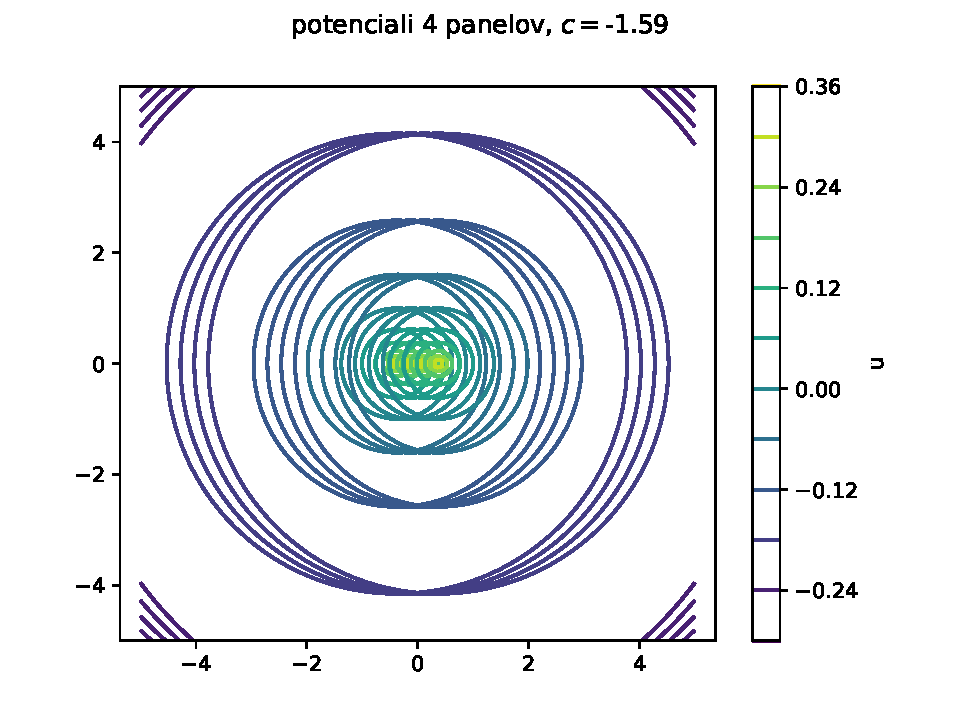
\includegraphics[width=0.6\textwidth]{9.nal_slike/doprinos_panelov.pdf}
    \caption{Potenciali panelov prikazani posebej}
\end{figure}

\begin{figure}[ht]
    \centering
    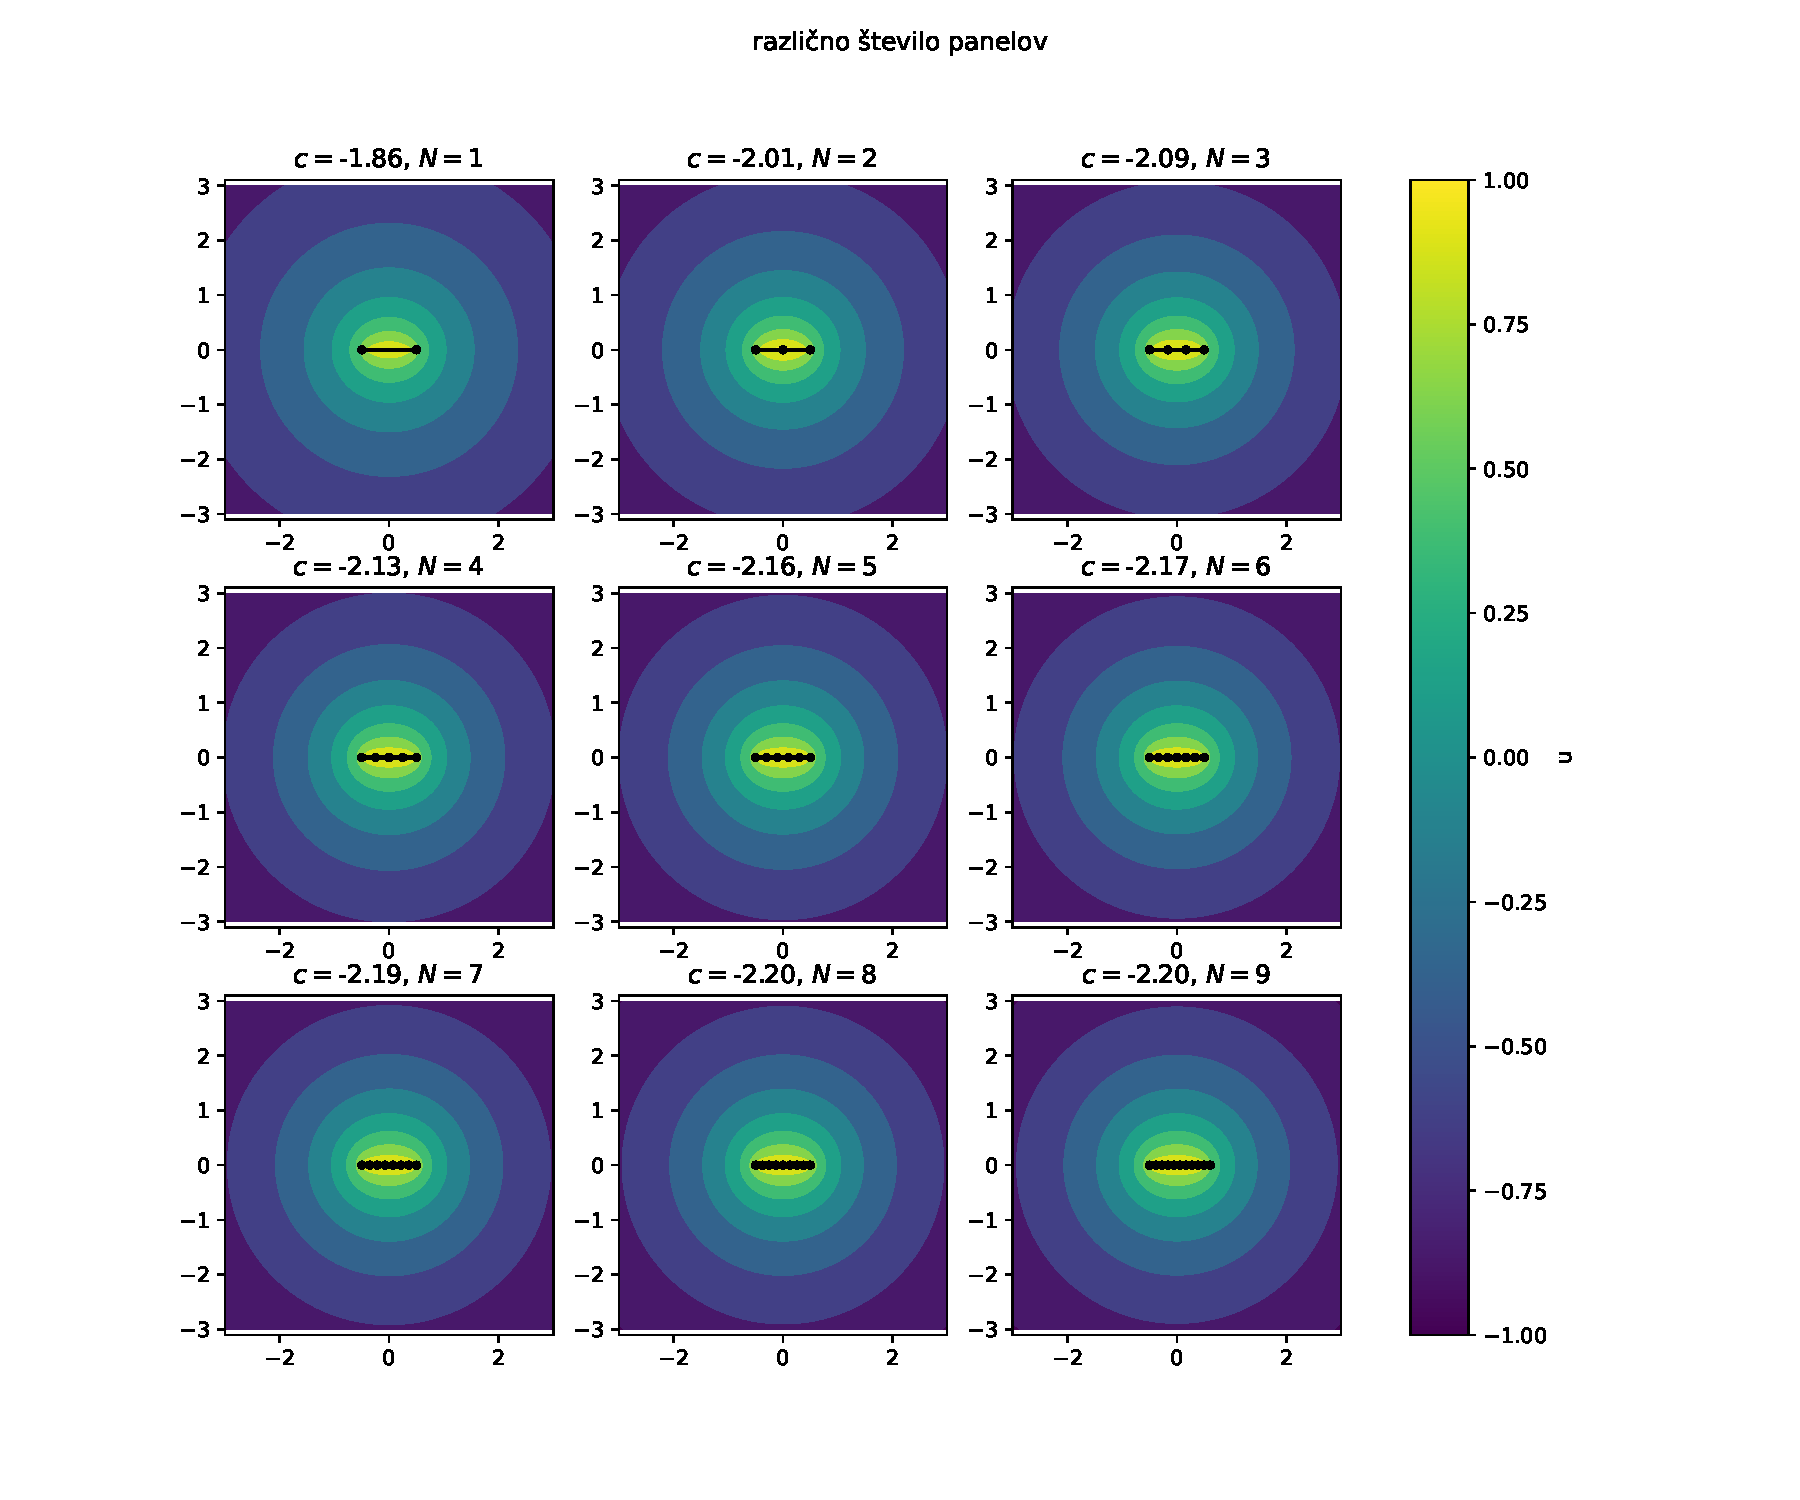
\includegraphics[width=\textwidth]{9.nal_slike/vodoravni_paneli.pdf}
    \caption{Vodoraven nabit trak}
\end{figure}

Pri tem opazim, da se (nelinearno) spreminja tudi kapaciteta elektrode $c$, zato izvedem več izračunov in primerjam rezultat. Pričakovano rešitev konvergira, in sicer k vrednosti blizu $-2.25$, vendar lahko rečem, da že z cca. 30 paneli dovolj dobro popišemo probem.
\begin{figure}[H]
    \centering
    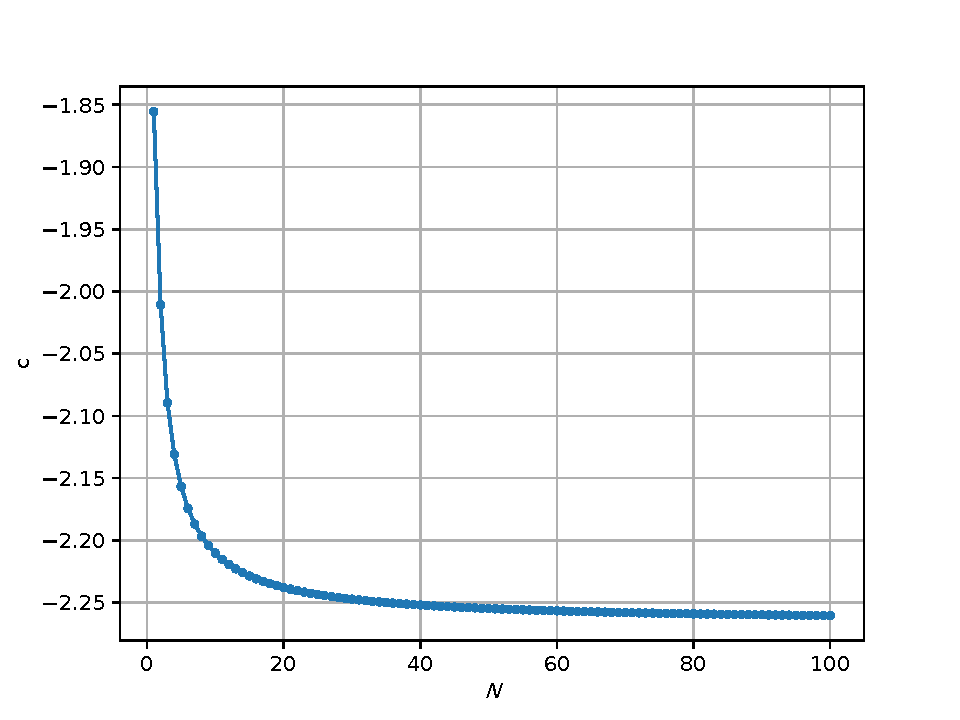
\includegraphics[width=0.47\textwidth]{9.nal_slike/kapciteta_vodoravni_paneli.pdf}
    \caption{Kapaciteta elektrode - konvergenca}
\end{figure}

Relativno preprosto je tudi natak način pridobiti gostoto naboja, saj je le-to rešitev sistema enačb. tako prikažem na sliki spodaj porazdelitev naboja po dolgem nabitem vodoravnem traku širine 1. Tudi iz te slike je lepo vidna konvergenca rešitve, vendar že z majhnim številom panelov presenetljivo dobro popišemo sistem.

\begin{figure}[ht]
    \centering
    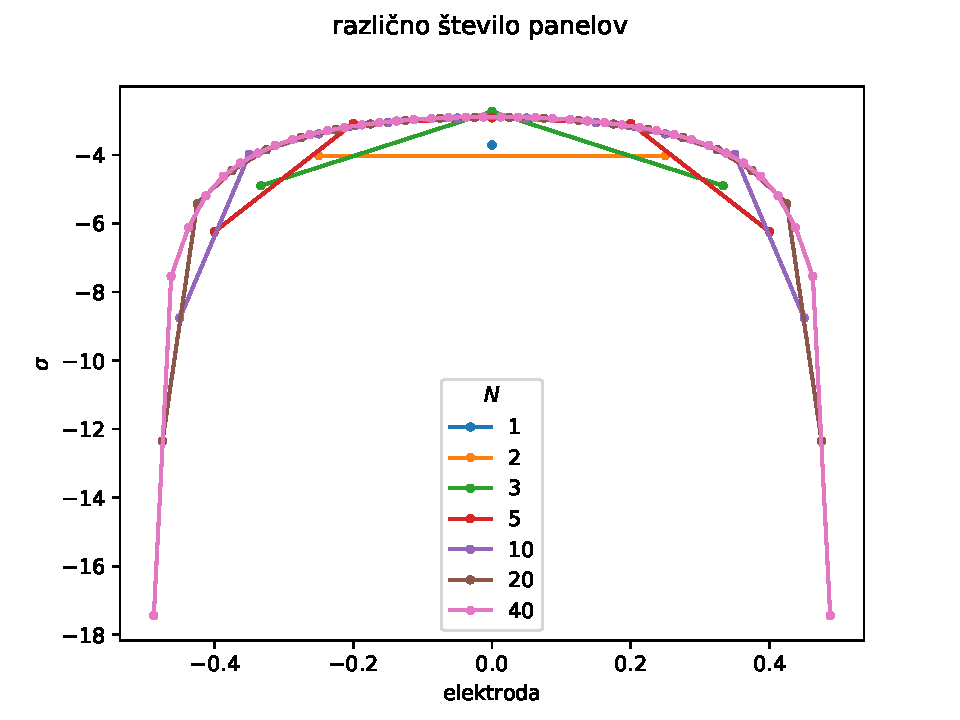
\includegraphics[width=0.7\textwidth]{9.nal_slike/sigma_plosca.pdf}
    \caption{Porazdelitev naboja po elektrodi}
\end{figure}

Preizkusil sem tudi, kakšno je polje okoli ravnega, vandar tokrat poševnega nabitega traku. Rezultat je v daljnem polju popolnoma enak kot prej, takisto tudi porazdelitev naboja. Bližnje polje pa dokazuje, da sem pravilno implementiral zasuk.

\begin{figure}[ht]
    \centering
    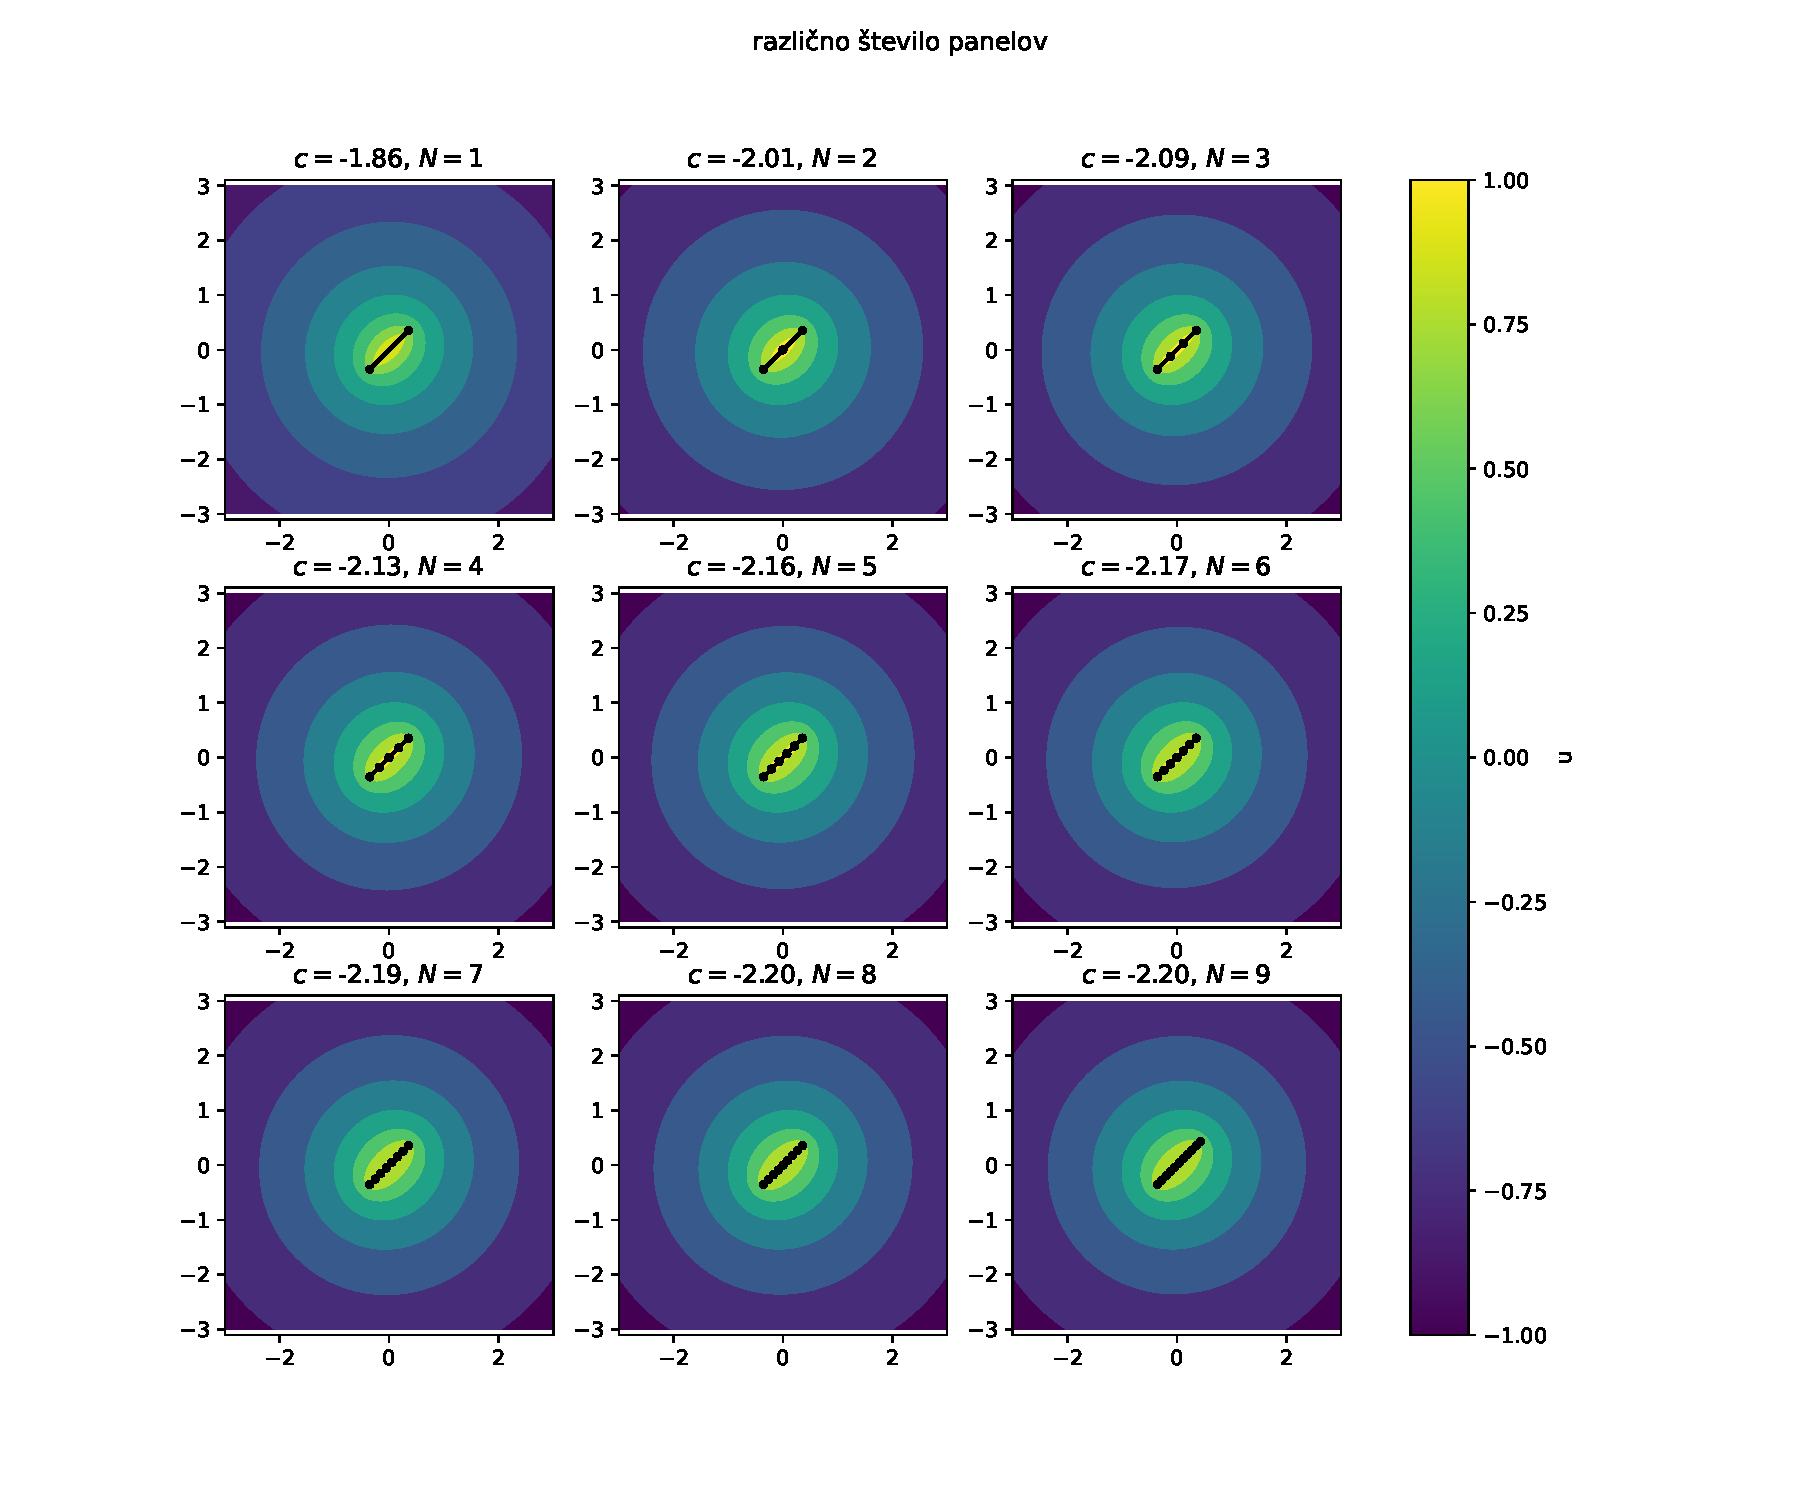
\includegraphics[width=\textwidth]{9.nal_slike/posevni_paneli.pdf}
    \caption{Poševen (45$^\circ$) nabit trak}
\end{figure}

\FloatBarrier
    \subsection{Različne oblike elektrod}

Ker metoda lepo deluje, preizkusim še nekaj bolj kompleksnih (sklenjenih) oblik, kot so krog, trikotnik in kvadrat. Pričakovano je naboj po krogu konstanten, prav tako tudi polje znotraj kroga, polje pa že nedaleč proč kot polje točkovnega naboja. To se zgodi že pri razmeroma majhnem št. panelov $N$. Malenkost presenetljivo pa je, da v tem primeru ne opazim konvergence kapacitivnosti, še bolj čudno je, da narašča nelinearno, in sicer v negativno vrednost!

Pri trikotni elektrodi je polje podobno okrogli, z razliko v bližjem polju, medtem ko je v ogliščih povečana gostota naboja, kar se opazi že pri mlo panelih ($N=9$). V tem primeru pa je opazna konvergenca kapacitivnosti!

Kvadratna elektroda ponovno povzrača nekaj težav, saj je v tem primeru polje ravno obrnjeno, čeravno sem uporabljal isto kodo in generiral točke na enak način in v isti smeri kot pri trikotniku! rezulati imajo vseeno smiselno obliko, v tem primeru pa polja znotraj elektrode sploh ni.

\begin{figure}[ht]
    \centering
    \begin{subfigure}{\textwidth}
        \centering
        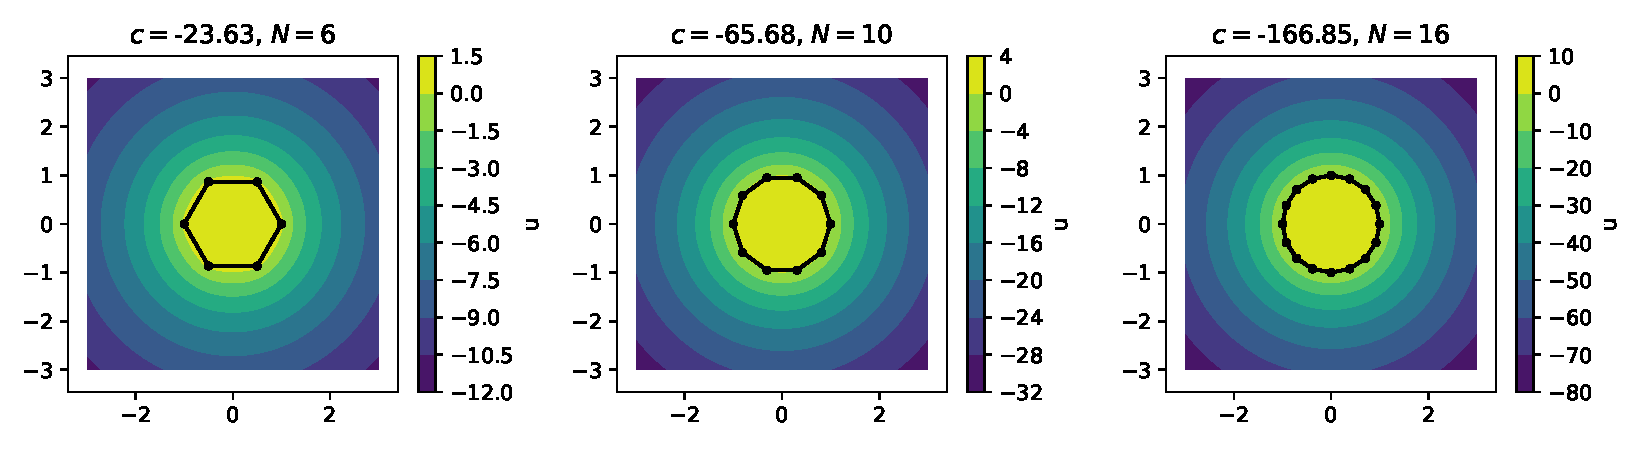
\includegraphics[width=\linewidth]{9.nal_slike/paneli_oblike/krog.pdf}
        \caption{Potencial}
    \end{subfigure}
    \begin{subfigure}{0.5\textwidth}
        \centering
        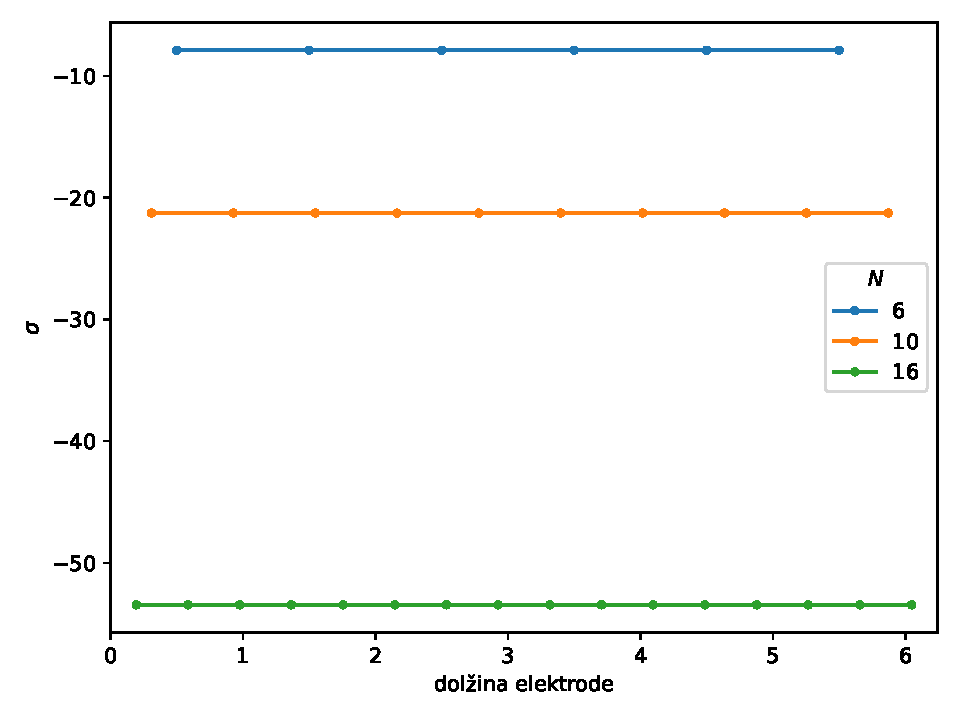
\includegraphics[width=\linewidth]{9.nal_slike/paneli_oblike/krog_sigma.pdf}
        \caption{Gostota naboja}
    \end{subfigure}
    \caption{Okrogla elektroda}
\end{figure}

\begin{figure}[ht]
    \centering
    \begin{subfigure}{\textwidth}
        \centering
        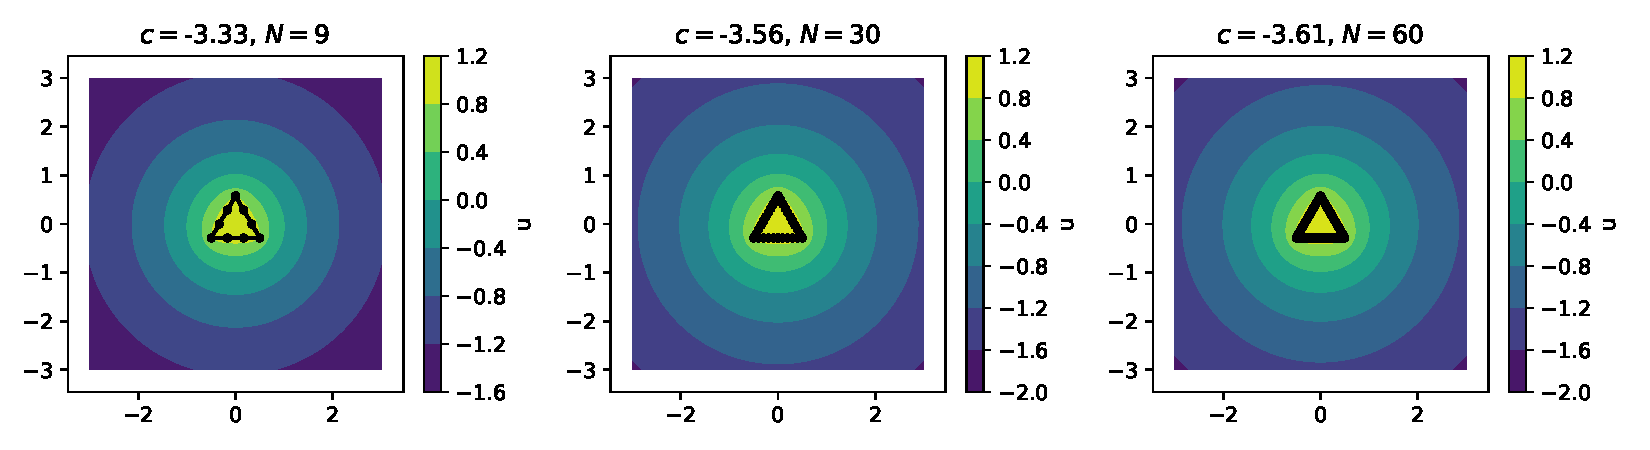
\includegraphics[width=\linewidth]{9.nal_slike/paneli_oblike/trikot.pdf}
        \caption{Potencial}
    \end{subfigure}
    \begin{subfigure}{0.5\textwidth}
        \centering
        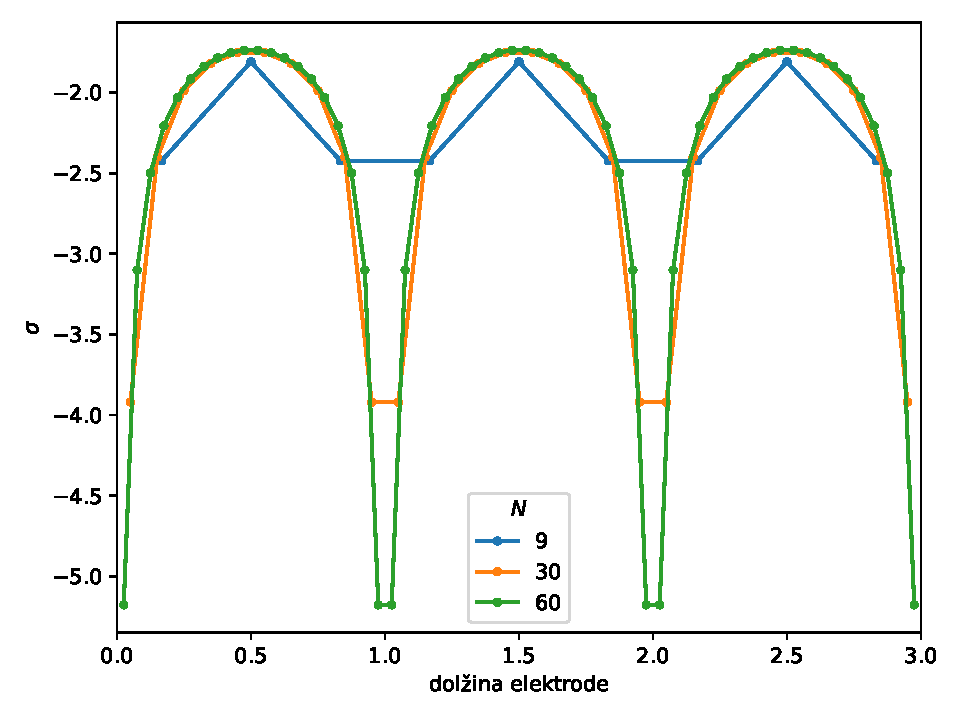
\includegraphics[width=\linewidth]{9.nal_slike/paneli_oblike/trikot_sigma.pdf}
        \caption{Gostota naboja}
    \end{subfigure}
    \caption{Trikotna elektroda}
\end{figure}

\begin{figure}[H]
    \centering
    \begin{subfigure}{\textwidth}
        \centering
        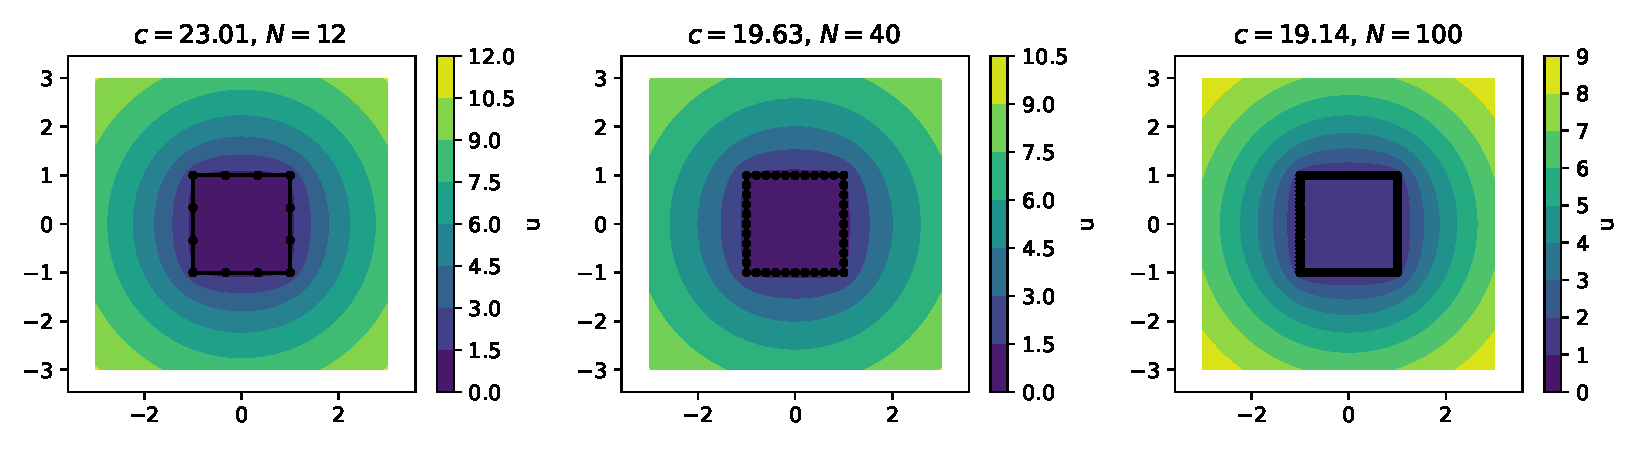
\includegraphics[width=\linewidth]{9.nal_slike/paneli_oblike/kvadrat.pdf}
        \caption{Potencial}
    \end{subfigure}
    \begin{subfigure}{0.5\textwidth}
        \centering
        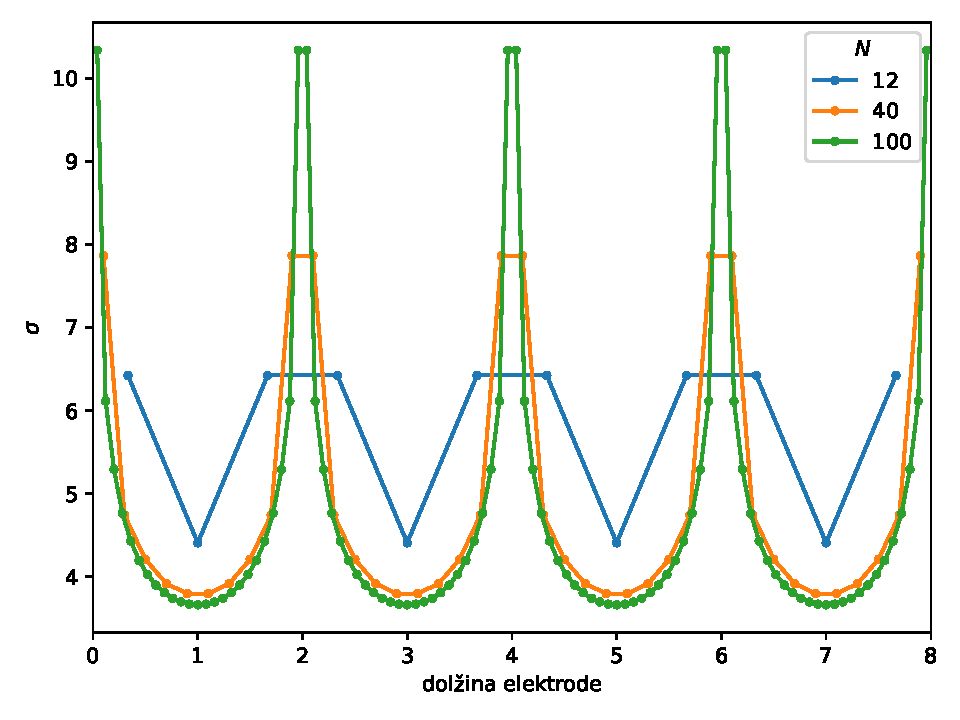
\includegraphics[width=\linewidth]{9.nal_slike/paneli_oblike/kvadrat_sigma.pdf}
        \caption{Gostota naboja}
    \end{subfigure}
    \caption{Kvadratna elektroda}
\end{figure}

\newpage
Za konec sem poizkusil še nesklenjeno elektrodo, ki pa ima ponovno čudne lastnosti kvadrata, čeravno je porazdelitev naboja prave oblike, saj je večje koncentracija pričakovana na prostih robovih.

\begin{figure}[ht]
    \begin{subfigure}{0.49\textwidth}
        \centering
        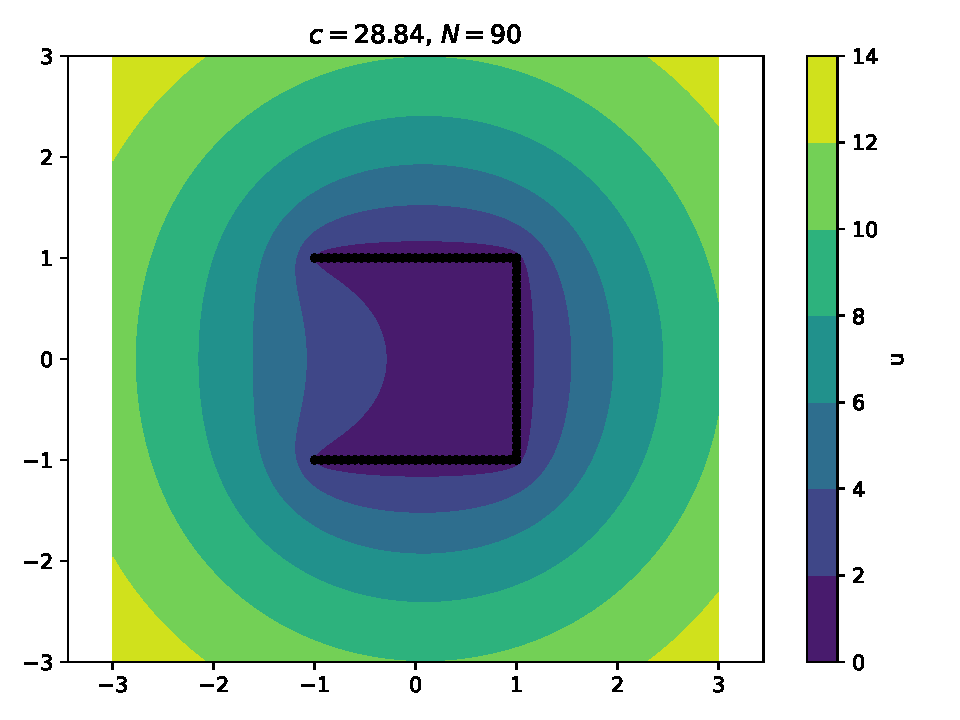
\includegraphics[width=\linewidth]{9.nal_slike/paneli_oblike/odprt_kvadrat.pdf}
        \caption{polje}
    \end{subfigure}
    \begin{subfigure}{0.49\textwidth}
        \centering
        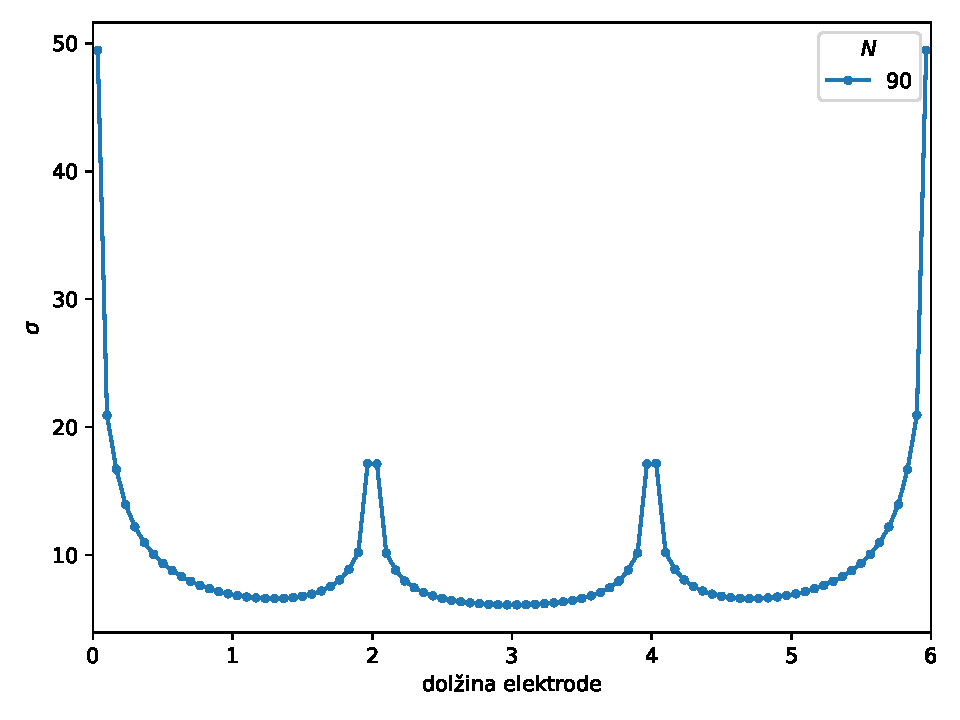
\includegraphics[width=\linewidth]{9.nal_slike/paneli_oblike/odprt_kvadrat_sigma.pdf}
        \caption{porazdelitev naboja}
    \end{subfigure}
    \caption{Odprta kvadratna elektroda}
\end{figure}

Dvojni krog ima enake lastnosti kot enojni, le vrednosti potenciala so višje. zanimivo pa postane, ko dodam povezovalni element med krogoma, ki močno zmoti polje. Očitno imajo taka nesimetrična vpetja lahko velik vpliv na polje!

\begin{figure}[ht]
    \centering
    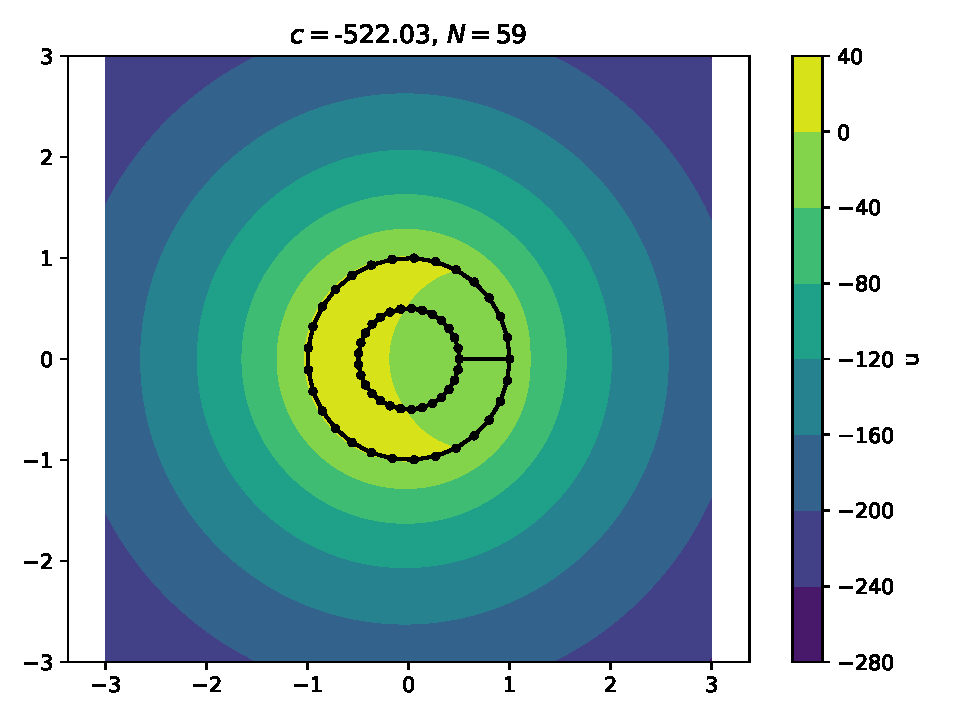
\includegraphics[width=0.5\linewidth]{9.nal_slike/paneli_oblike/krog_dva.pdf}
    \caption{Dvojni krog - polje}
\end{figure}


\FloatBarrier
\section{Hidrodinamika}

V tem primeru rešujem problem obtekanja teles s potencialnim tokom in sem tvoril sistem enačb
\begin{equation}
    V_{ij}^{\perp}\,\sigma_j = -v_{i,\infty}^{\perp},
\end{equation}
kjer je $V_{ij}^{\perp}$ doprinos potenciala j-tega panela na mestu i-tega panelav normalni(pravokotni) smeri, $v_{i,\infty}^{\perp}$ komponenta hitrosti v neskončnosti, ki je pravokotna na i-ti panel in $\sigma_j$ neznane vrednosti izvorov hitrostnega polja v j-tem panelu. Poznamo fundamentalni rešitvi za normalno $v_{\perp}$ in tangencialno $v_{\parallel}$ komponento hitrosti v lokalnem KS vsakega panela, katere je potrebno nato transformirati v željeni koordinatni sistem (globalni ali drugega panela).

Kot prvo rešujem problem obtekanja elipsoida z razmerjem glavnih osi v y- in x-osi $b$
\begin{equation}
    x=\cos{\varphi}, \quad y=b\,\sin{\varphi},
\end{equation}
ki je v najenostvnejšem primeru, ko $b=1$, krožnica. Za take preproste oblike poznamo analitično rešitev tangencialne komponente hitrosti ob robu elipsoida, kjer iz robnih pogojev sicer vemo, da $v_{\perp}=0$,
\begin{equation}
    v_{\parallel} = v_{\infty}^{\parallel} \,\frac{(1+b)\,y}{\sqrt{y^2+b^4\,x^2}}.
\end{equation}

Izračunal sem na tak način hitrostno polje okoli dolgega valja, ki se poenostavi v ravninski problem obtekanja okoli kroga. Zaradi osne simetrije je v tem primeru polje hitrosti neodvisno od smeri (vpadnega kota), kar je razvidno iz tokovnic na spodnji sliki. Za primer vodoravnega toka -- vpadnega kota 0 -- sem izračunal tudi vzporedno komponento hitrosti tik ob panelu, ki sem jo lahko primerjal z analitično. Zaradi singularnosti sem računal v točki za $10^{-10}$ odmaknjene od središča panela. Rezultat je presenetljiv, saj izgleda, da izračunana hitrost linearno pada in pri $N=41$ doseže optimum, saj je residual reda $10^{-3}$, rešitev pa je na pogled enaka analitični.

V vseh spodnjih primerih so rešitve prikazane v obliki tokovnic, kjer sem pozkušal izločiti polje znotraj elipse, vendar je to povzročilo prekinitev tokovnic, ki jih izrisuje program. Prav tako sem tangencialno hitrost na površini računal za primer vodoravnega toka.

\begin{figure}[ht]
    \centering
    \begin{subfigure}{0.49\textwidth}
        \centering
        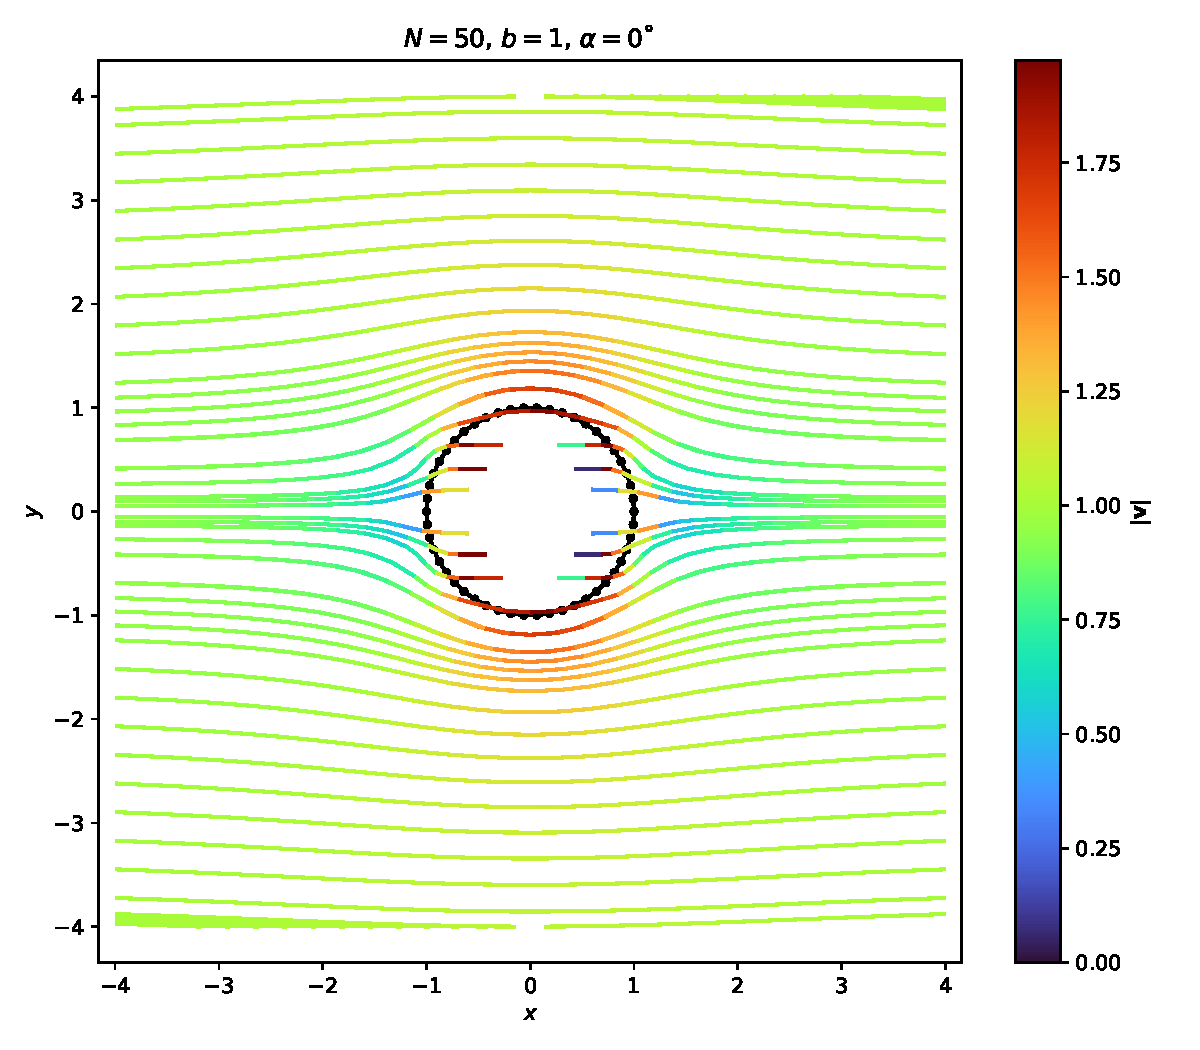
\includegraphics[width=\linewidth]{9.nal_slike/hidro/b1_N50_alpha0.pdf}
        \caption{Vodoraven tok}
    \end{subfigure}
    \begin{subfigure}{0.49\textwidth}
        \centering
        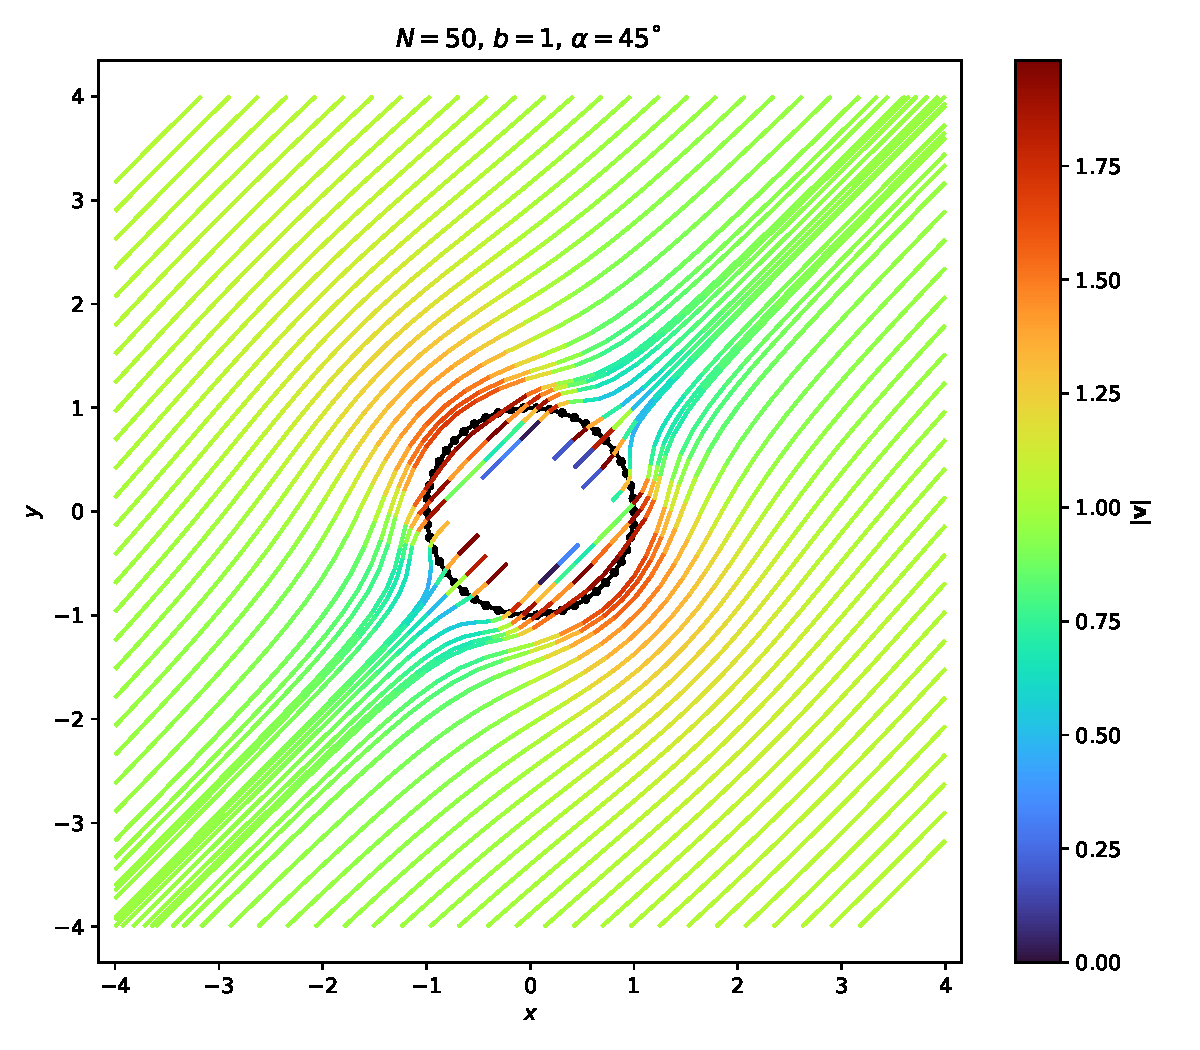
\includegraphics[width=\linewidth]{9.nal_slike/hidro/b1_N50_alpha45.pdf}
        \caption{Tok pod 45$^\circ$}
    \end{subfigure}
    \begin{subfigure}{0.49\textwidth}
        \centering
        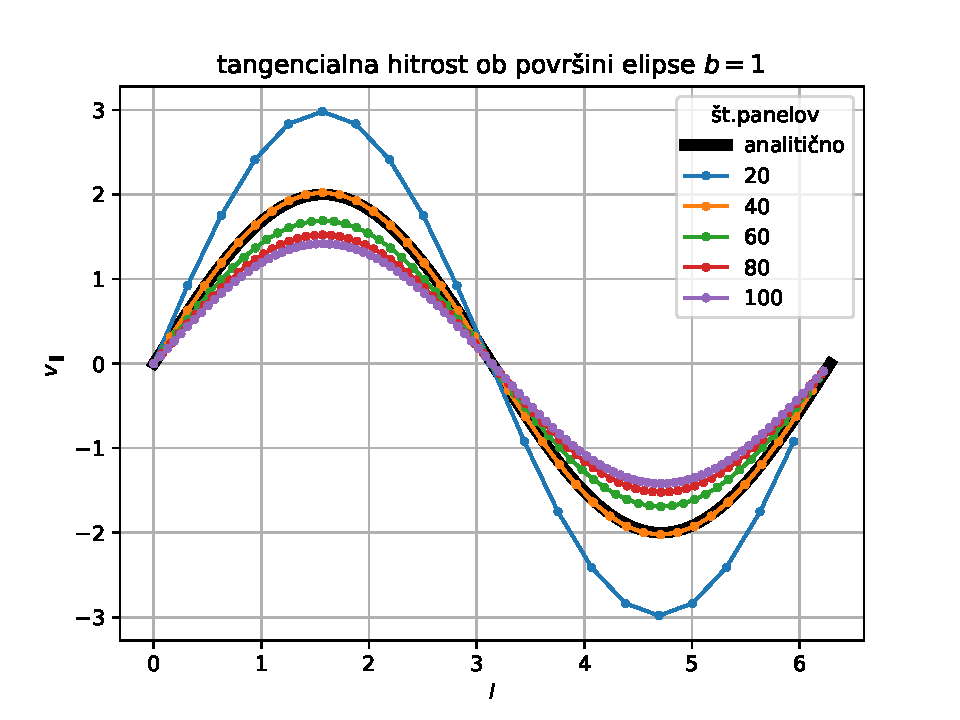
\includegraphics[width=\linewidth]{9.nal_slike/hidro/vt_b1.pdf}
        \caption{Primerjava z analitično rešitvijo}
    \end{subfigure}
    \begin{subfigure}{0.49\textwidth}
        \centering
        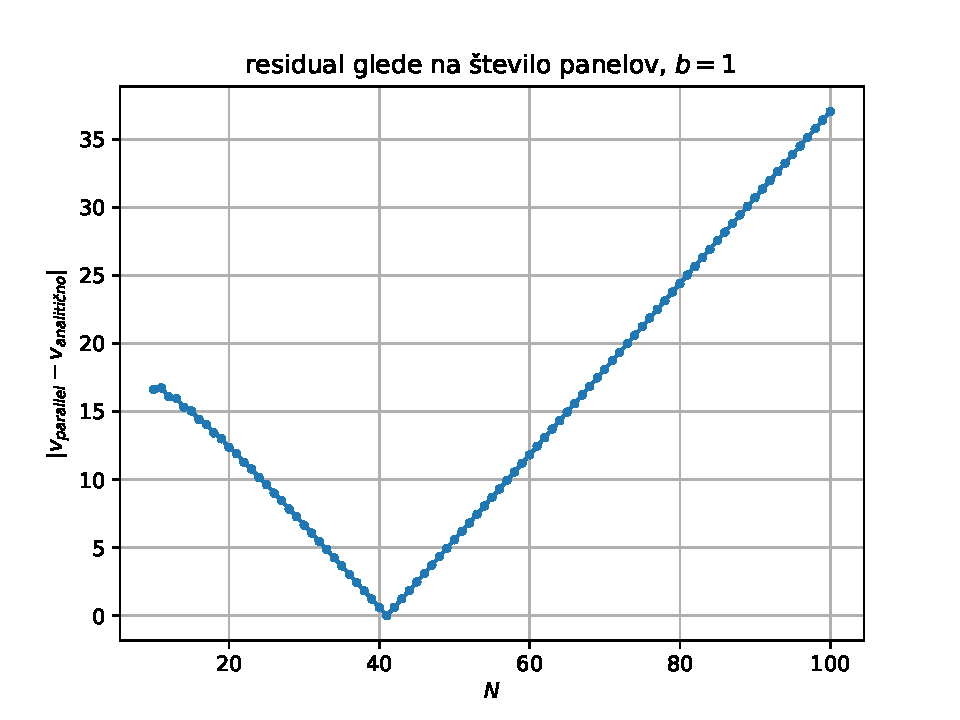
\includegraphics[width=\linewidth]{9.nal_slike/hidro/residual_b1.pdf}
        \caption{Odstopanje od analitične rešitve}
    \end{subfigure}
    \caption{Obtekanje kroga $b=1$}
\end{figure}

Ko spremenim parameter $b$, problem postane anizotropen, zato v takem primeru vpadni kot tekočine igra pomembno vlogo pri hitrostnem polju. 

Opazim, da v tem primeru metoda slabše popiše analitičen potek hitrosti, saj tudi v optimalni točki še vedno obsataja večji residual kot prej. Vseeno pa, vsaj pri manjših razmerjih polosi $b$, še vedno obstaja optimum, vendar potek residuala ni več linearen. Pri večjih $b$ in pri $b \rightarrow 0$ metoda vse slabše popiše potek in postaja nestabilna!

\begin{figure}[ht]
    \centering
    \begin{subfigure}{0.49\textwidth}
        \centering
        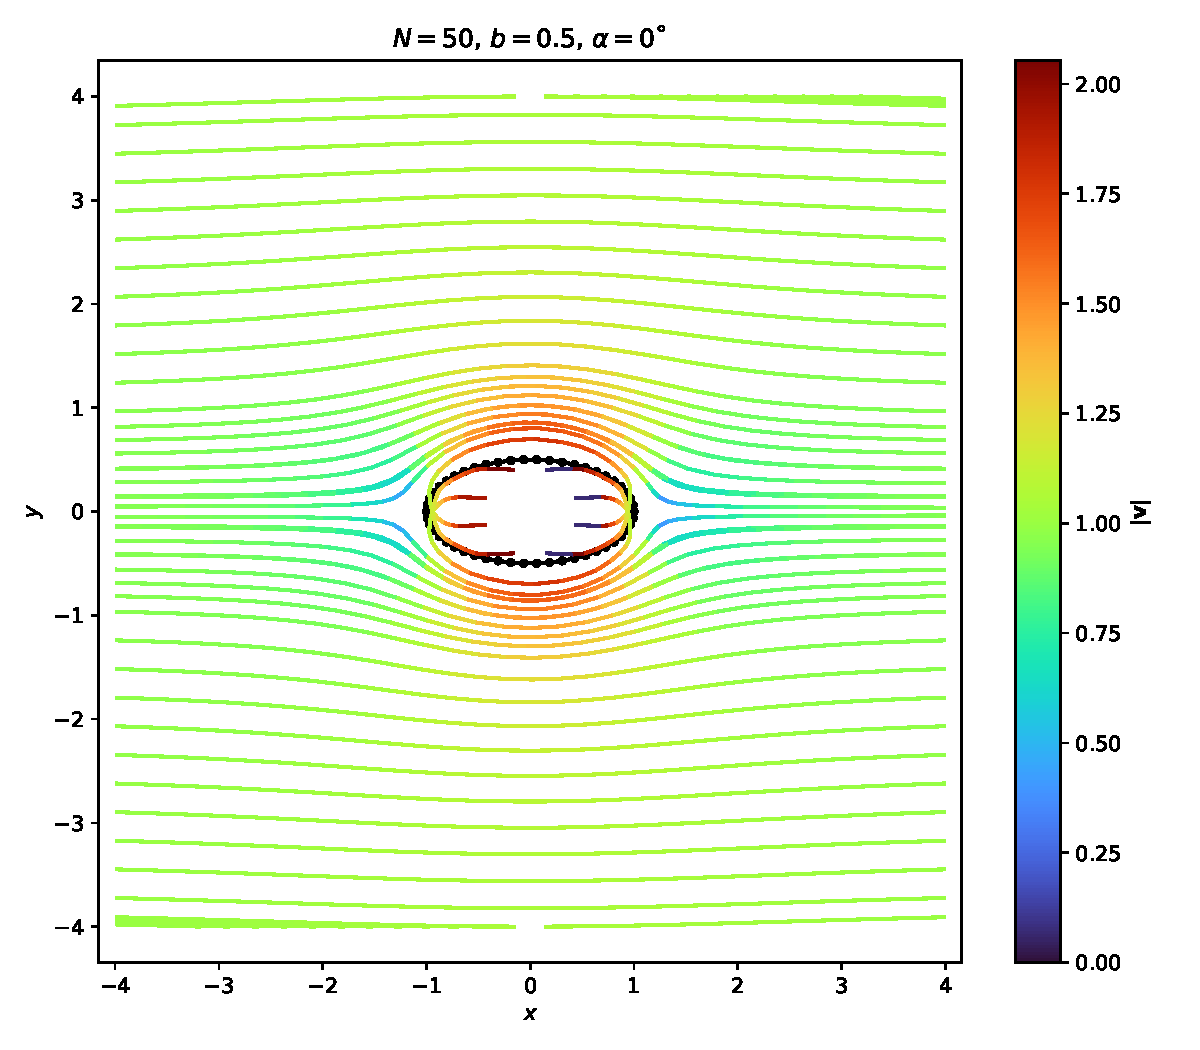
\includegraphics[width=\linewidth]{9.nal_slike/hidro/b0.5_N50_alpha0.pdf}
        \caption{Vodoraven tok}
    \end{subfigure}
    \begin{subfigure}{0.49\textwidth}
        \centering
        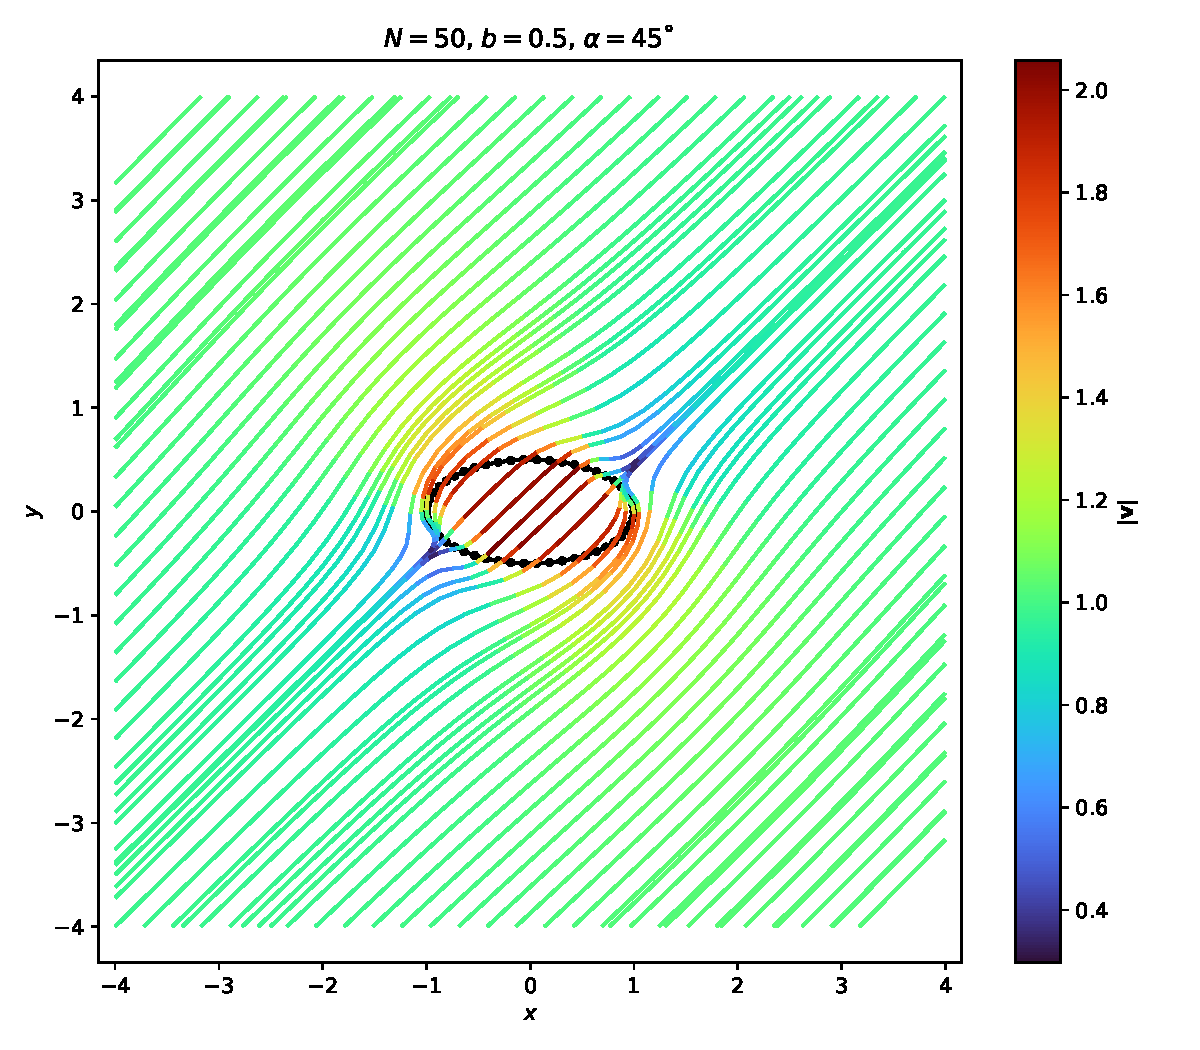
\includegraphics[width=\linewidth]{9.nal_slike/hidro/b0.5_N50_alpha45.pdf}
        \caption{Tok pod 45$^\circ$}
    \end{subfigure}
    \begin{subfigure}{0.49\textwidth}
        \centering
        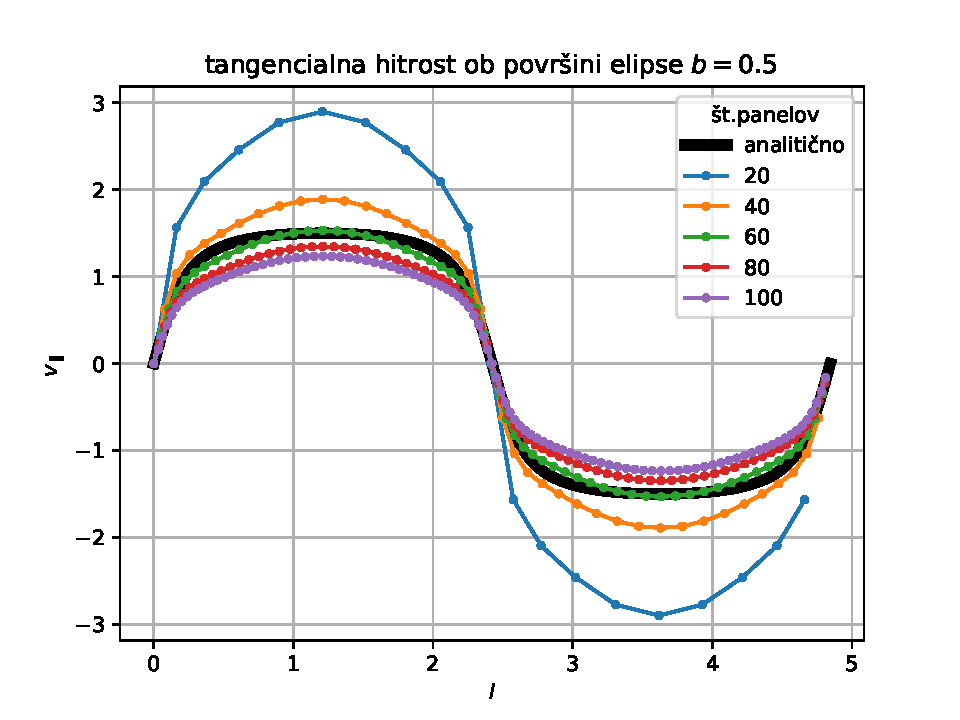
\includegraphics[width=\linewidth]{9.nal_slike/hidro/vt_b0.5.pdf}
        \caption{Primerjava z analitično rešitvijo}
    \end{subfigure}
    \begin{subfigure}{0.49\textwidth}
        \centering
        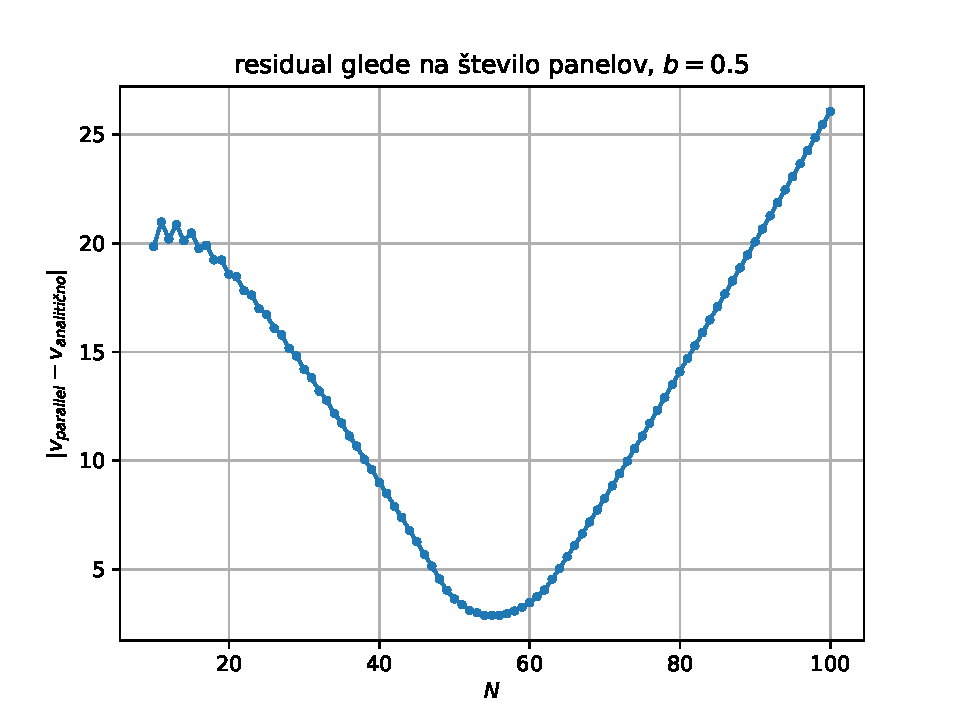
\includegraphics[width=\linewidth]{9.nal_slike/hidro/residual_b0.5.pdf}
        \caption{Odstopanje od analitične rešitve}
    \end{subfigure}
    \caption{Obtekanje elipse $b=0.5$}
\end{figure}

\begin{figure}[ht]
    \centering
    \begin{subfigure}{0.49\textwidth}
        \centering
        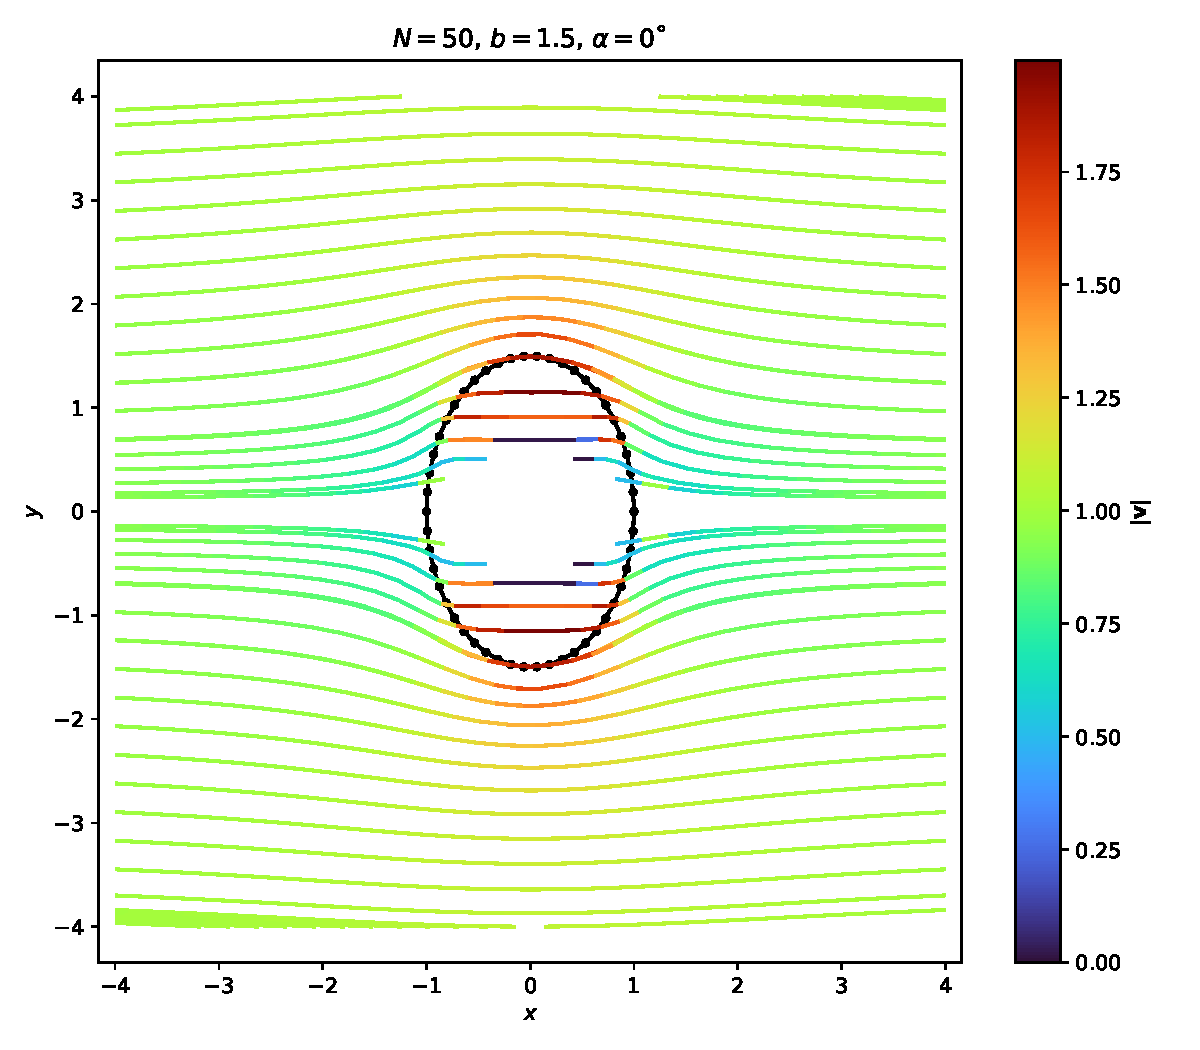
\includegraphics[width=\linewidth]{9.nal_slike/hidro/b1.5_N50_alpha0.pdf}
        \caption{Vodoraven tok}
    \end{subfigure}
    \begin{subfigure}{0.49\textwidth}
        \centering
        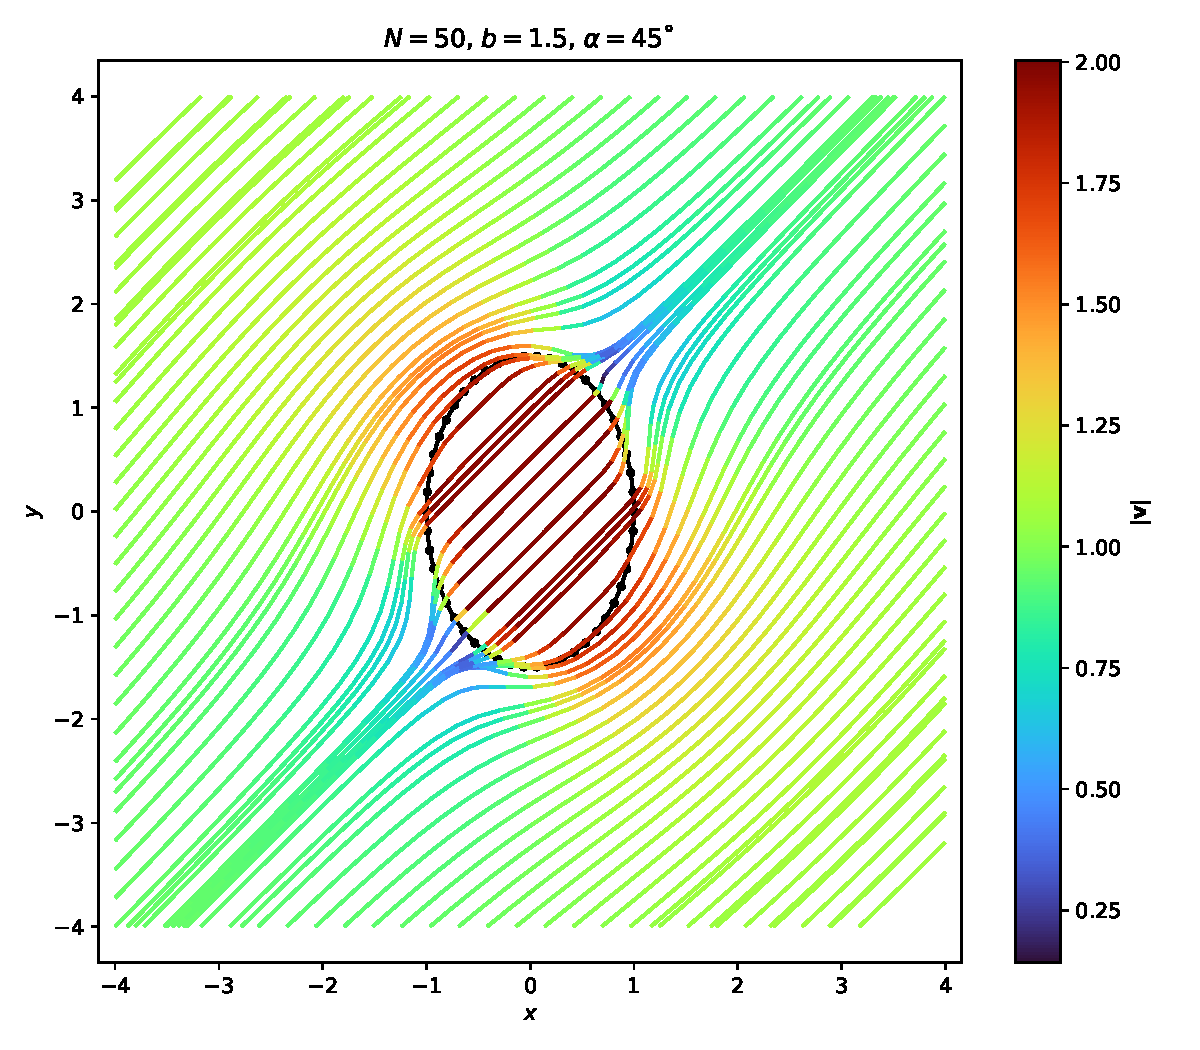
\includegraphics[width=\linewidth]{9.nal_slike/hidro/b1.5_N50_alpha45.pdf}
        \caption{Tok pod 45$^\circ$}
    \end{subfigure}
    \begin{subfigure}{0.49\textwidth}
        \centering
        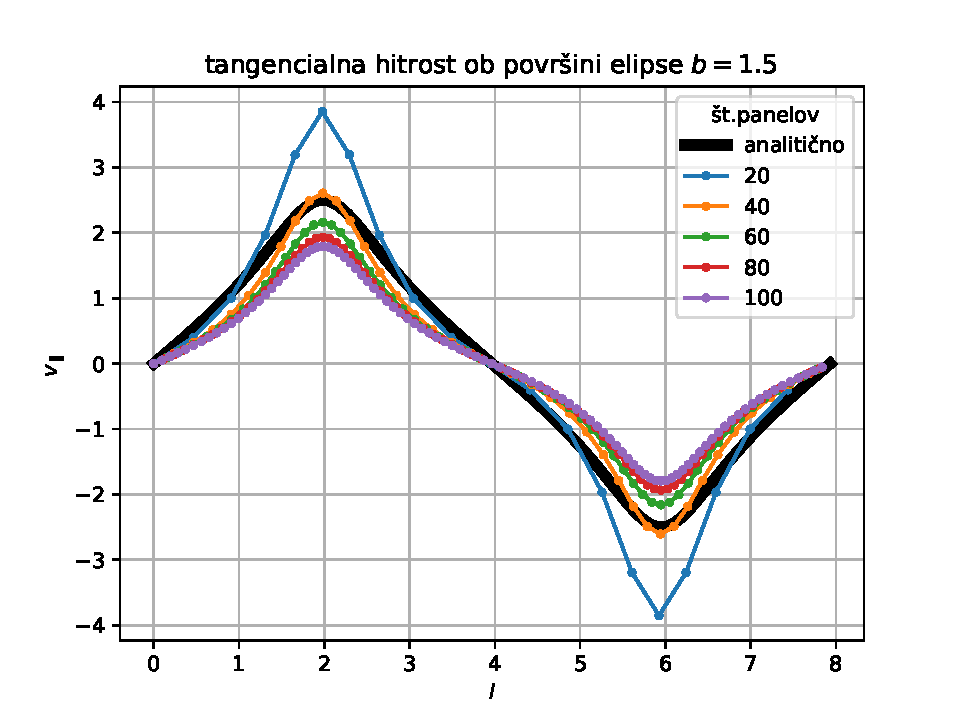
\includegraphics[width=\linewidth]{9.nal_slike/hidro/vt_b1.5.pdf}
        \caption{Primerjava z analitično rešitvijo}
    \end{subfigure}
    \begin{subfigure}{0.49\textwidth}
        \centering
        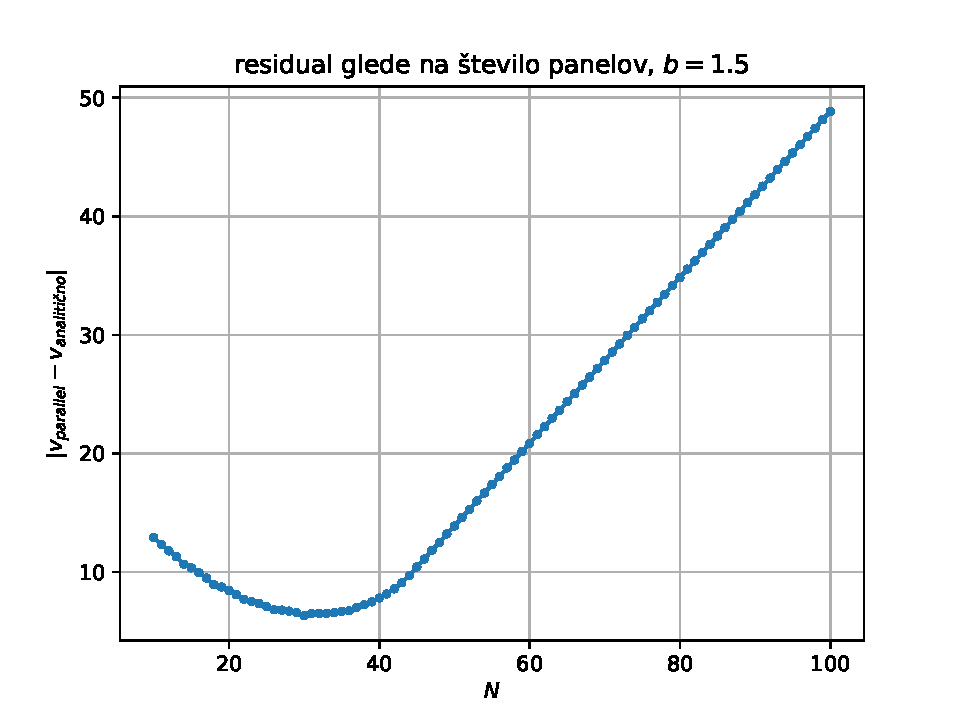
\includegraphics[width=\linewidth]{9.nal_slike/hidro/residual_b1.5.pdf}
        \caption{Odstopanje od analitične rešitve}
    \end{subfigure}
    \caption{Obtekanje elipse $b=1.5$}
\end{figure}

\begin{figure}[H]
    \centering
    \begin{subfigure}{\textwidth}
        \begin{subfigure}{0.49\textwidth}
            \centering
            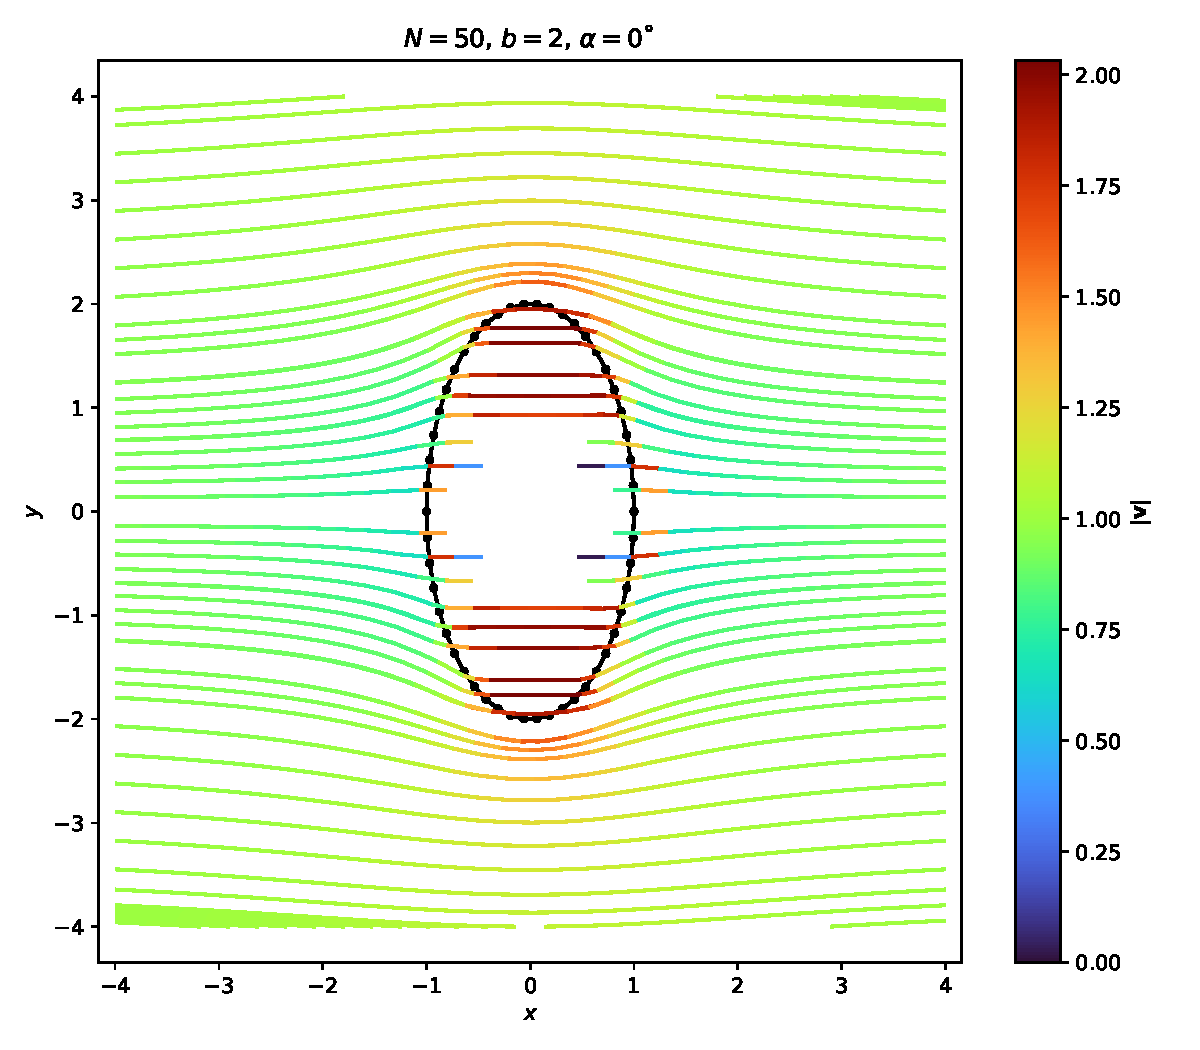
\includegraphics[width=\linewidth]{9.nal_slike/hidro/b2_N50_alpha0.pdf}
        \end{subfigure}
        \begin{subfigure}{0.49\textwidth}
            \centering
            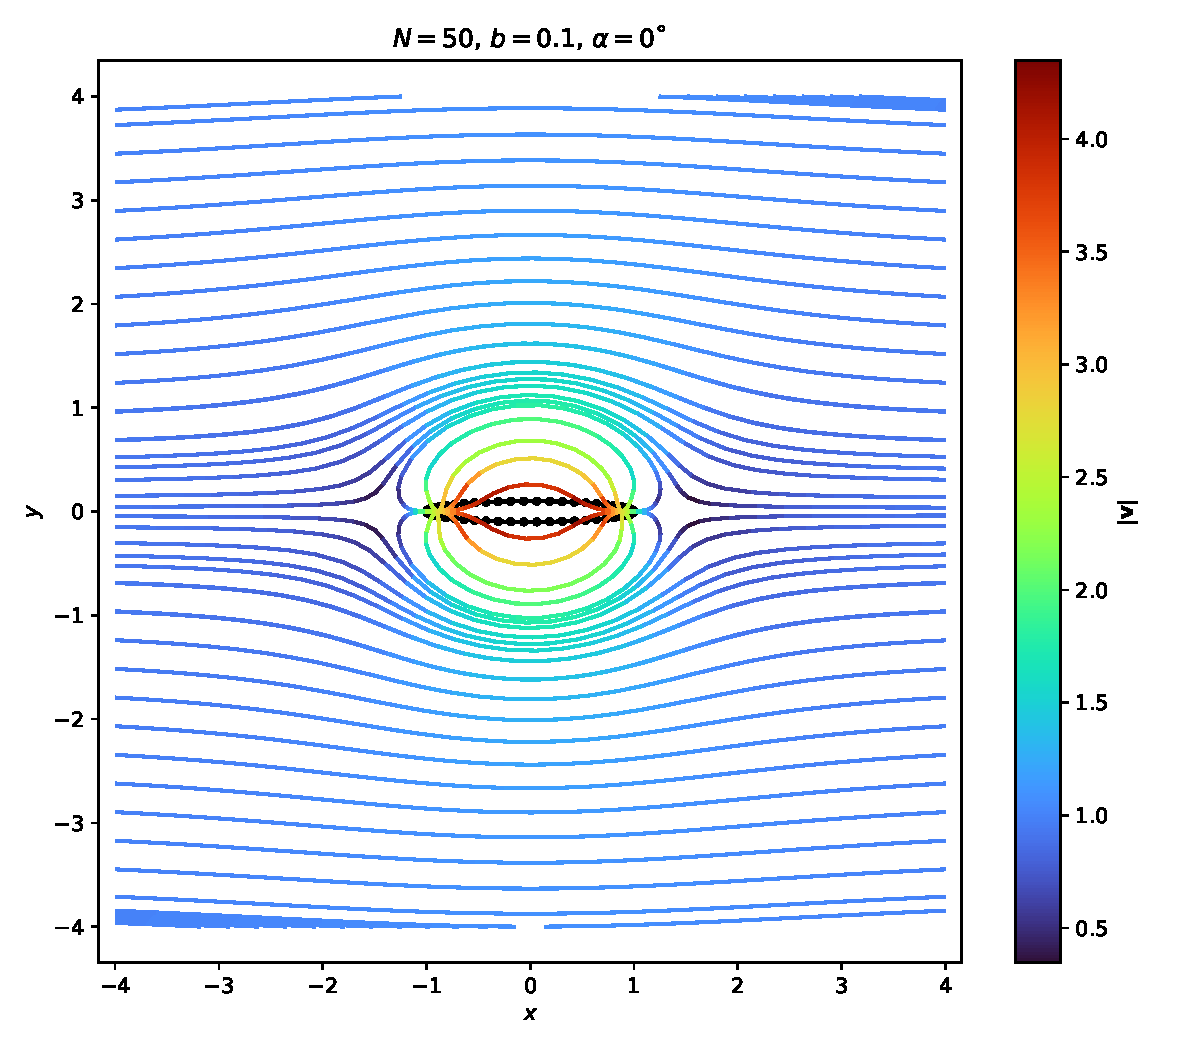
\includegraphics[width=\linewidth]{9.nal_slike/hidro/b0.1_N50_alpha0.pdf}
        \end{subfigure}
        \caption{Vodoraven tok}
    \end{subfigure}
    \begin{subfigure}{\textwidth}
        \begin{subfigure}{0.49\textwidth}
            \centering
            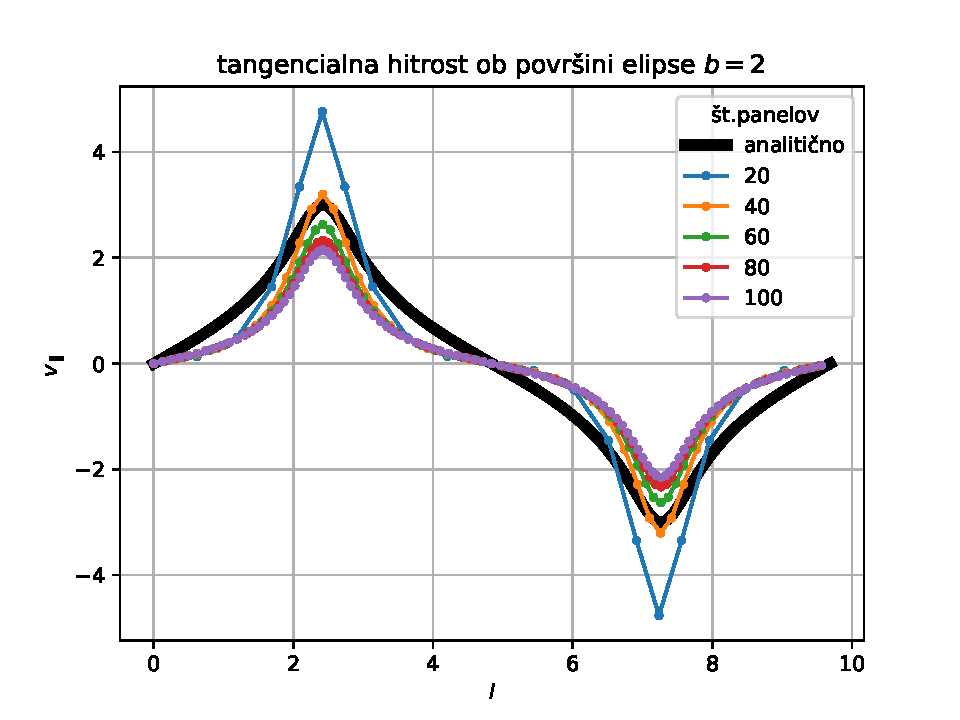
\includegraphics[width=\linewidth]{9.nal_slike/hidro/vt_b2.pdf}
        \end{subfigure}
        \begin{subfigure}{0.49\textwidth}
            \centering
            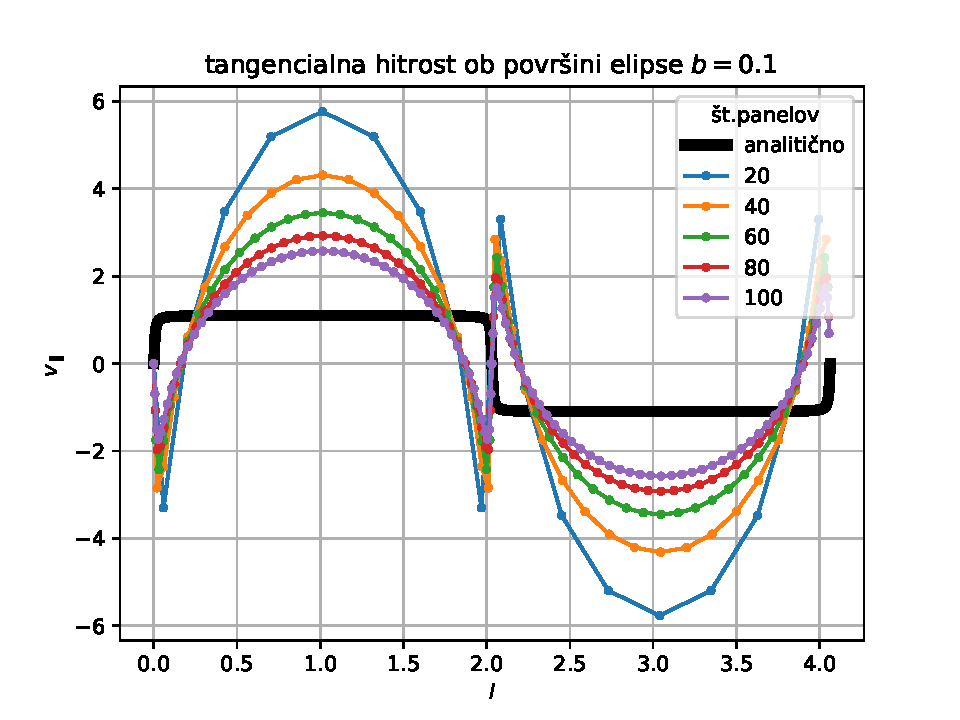
\includegraphics[width=\linewidth]{9.nal_slike/hidro/vt_b0.1.pdf}
        \end{subfigure}
        \caption{Primerjava z analitično rešitvijo}
    \end{subfigure}
    \begin{subfigure}{\textwidth}
        \begin{subfigure}{0.49\textwidth}
            \centering
            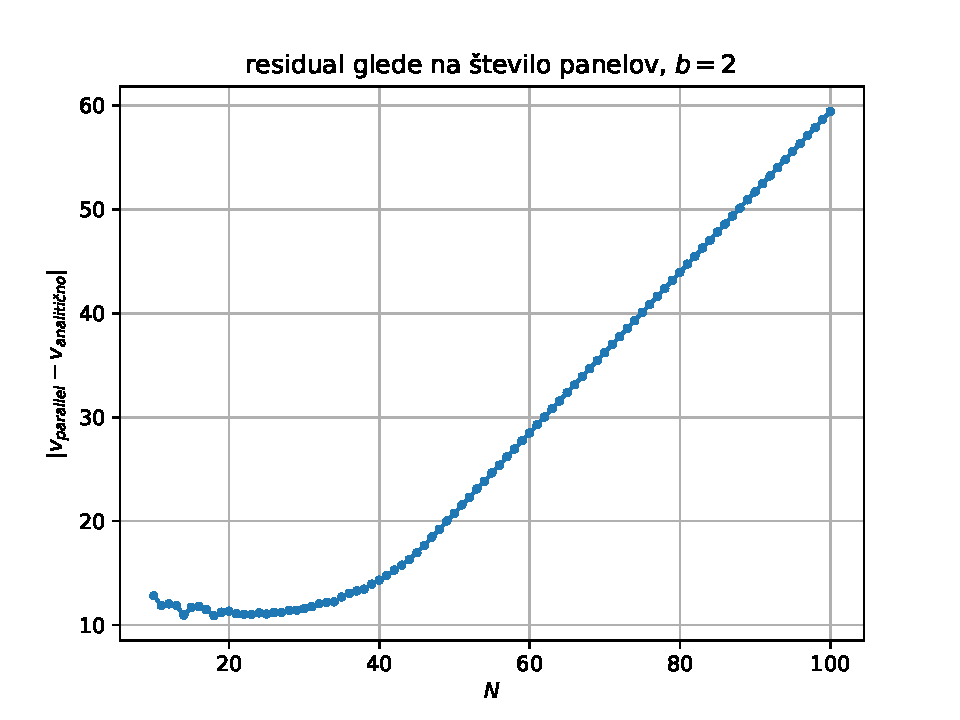
\includegraphics[width=\linewidth]{9.nal_slike/hidro/residual_b2.pdf}
        \end{subfigure}
        \begin{subfigure}{0.49\textwidth}
            \centering
            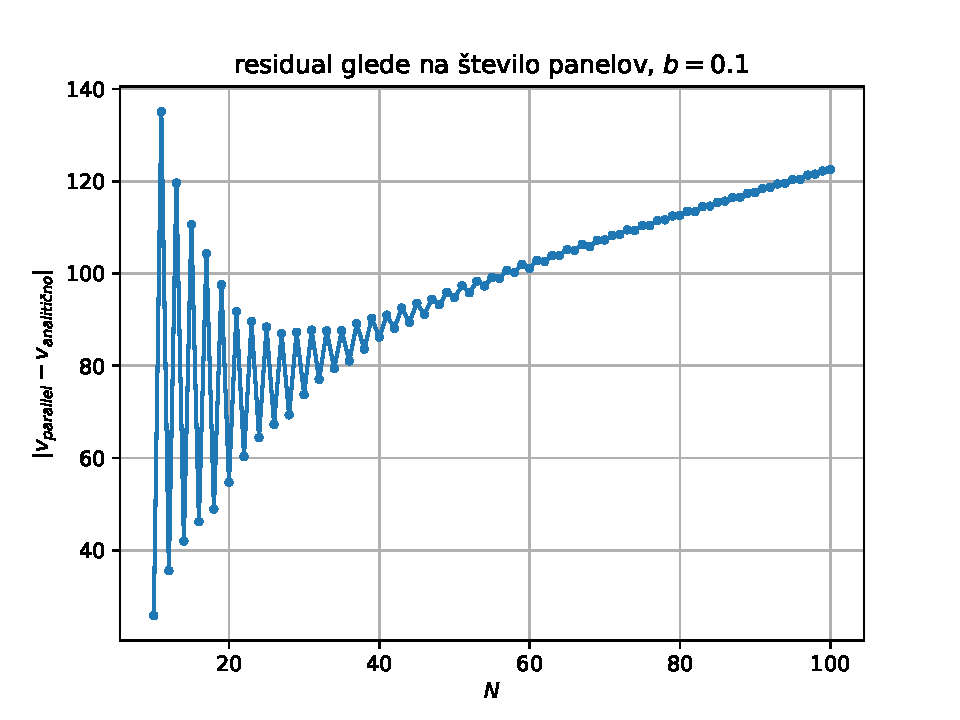
\includegraphics[width=\linewidth]{9.nal_slike/hidro/residual_b0.1.pdf}
        \end{subfigure}
        \caption{Odstopanje od analitične rešitve}
    \end{subfigure}
    \caption{Obtekanje elipse levo $b=2$, desno $b=0.1$}
\end{figure}

Primer slabe rešitve za $b \rightarrow 0$ je priakzan sicer že na zgornji sliki, vendar je pri večjem vpadnem kotu še bolj očiten. Fizikalno je sicer hitrost smiselna, vendar tik ob profilu popis ni ustrezen.

\begin{figure}[ht]
    \begin{center}
        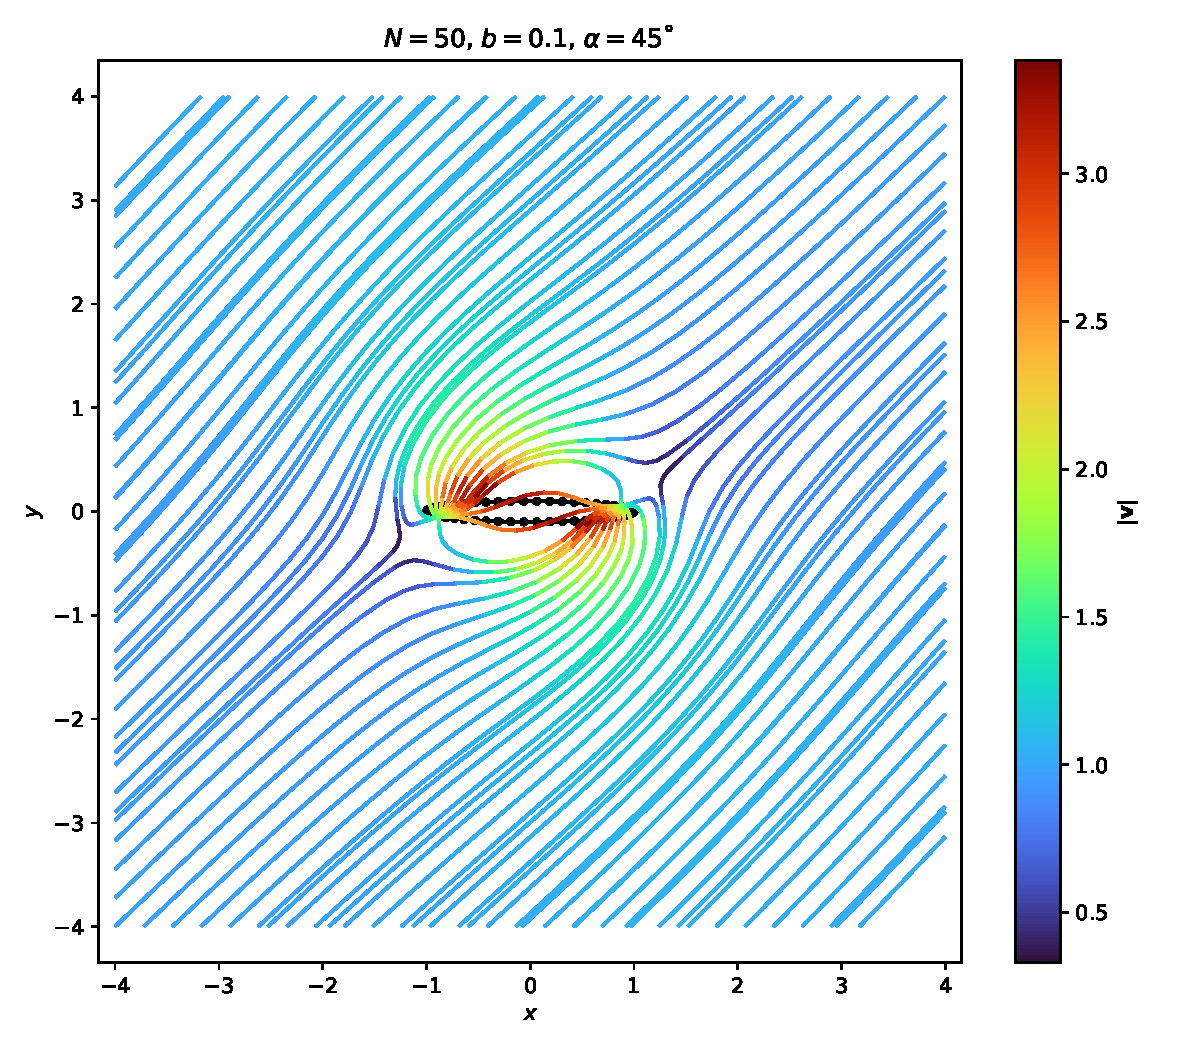
\includegraphics[width=0.5\linewidth]{9.nal_slike/hidro/b0.1_N50_alpha45.pdf}
    \end{center}
    \caption{degenerirana rešitev za $b=0.1$ in $\alpha=45^\circ$}
\end{figure}


\FloatBarrier
    \subsection{Obtekanje aeroprofila}

Metodo uprabim tudi za bolj realistične oblike, to so aeroprofili, katerih cilj je zmanjšanje zračnega upora pri čim večjem vzgonu. Kot prvo prikažem simetične NACA ``zero-camber'' aeroprofile, kjer lahko spreminjam le relativno debelino $t$. Enačba je podana v predlogi. Opazim podobno težavo, kot pri elipsah z $b \rightarrow 0$, saj za NACA-0010 metoda še solidno deluje, pri ostalih dveh primerih pa je degeneracije že močna. Tudi vektorsko polje hitrosti prikazuje, da rešitev ni popolnoma zadostila mojim fizikalnim pričakovanjem, kar je predvsem opazno pri povečanju vpadnega kota, v aeronavtiki se temu namreč reče ``angle of attack''.

\begin{figure}[H]
    \centering
    \begin{subfigure}{0.49\textwidth}
        \centering
        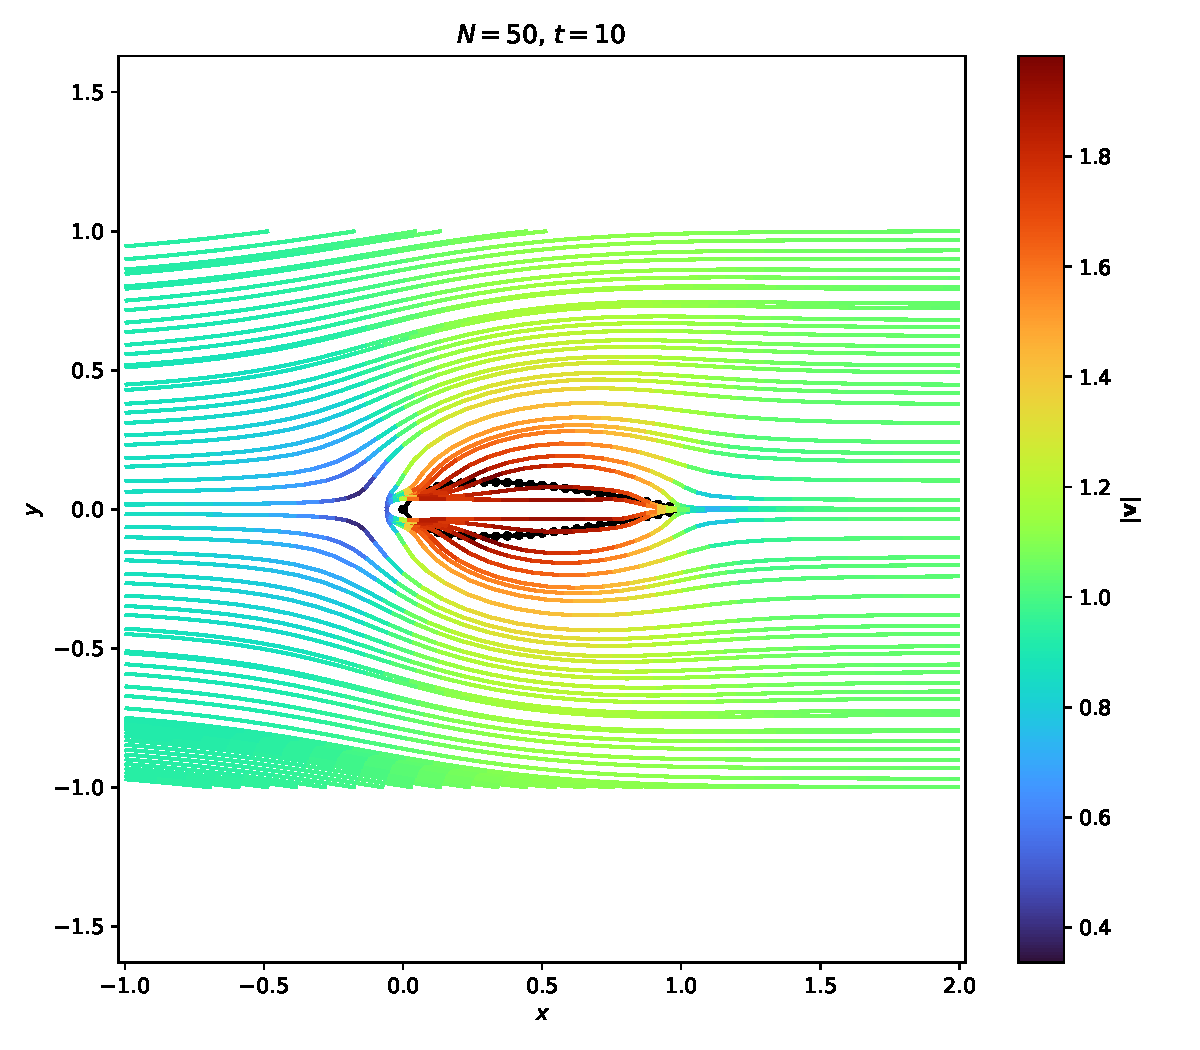
\includegraphics[width=\linewidth]{9.nal_slike/hidro/aeroprofil/NACA_t10_N50_alpha0.pdf}
        \caption{NACA-0010}
    \end{subfigure}
    \begin{subfigure}{0.49\textwidth}
        \centering
        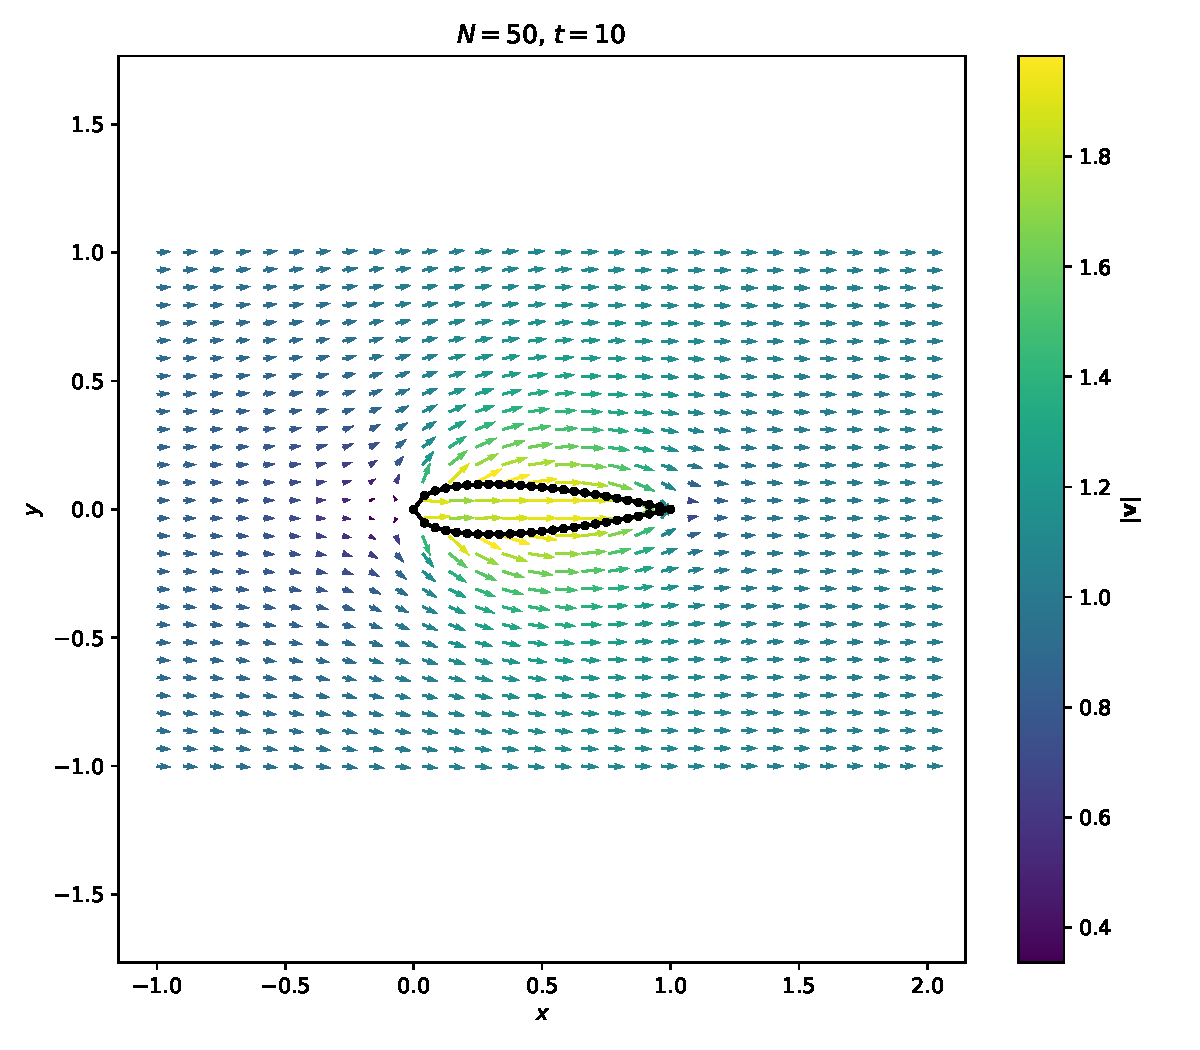
\includegraphics[width=\linewidth]{9.nal_slike/hidro/aeroprofil/NACA_vec_t10_N50_alpha0.pdf}
        \caption{NACA-0010, vekttorsko polje}
    \end{subfigure}
    \begin{subfigure}{0.49\textwidth}
        \centering
        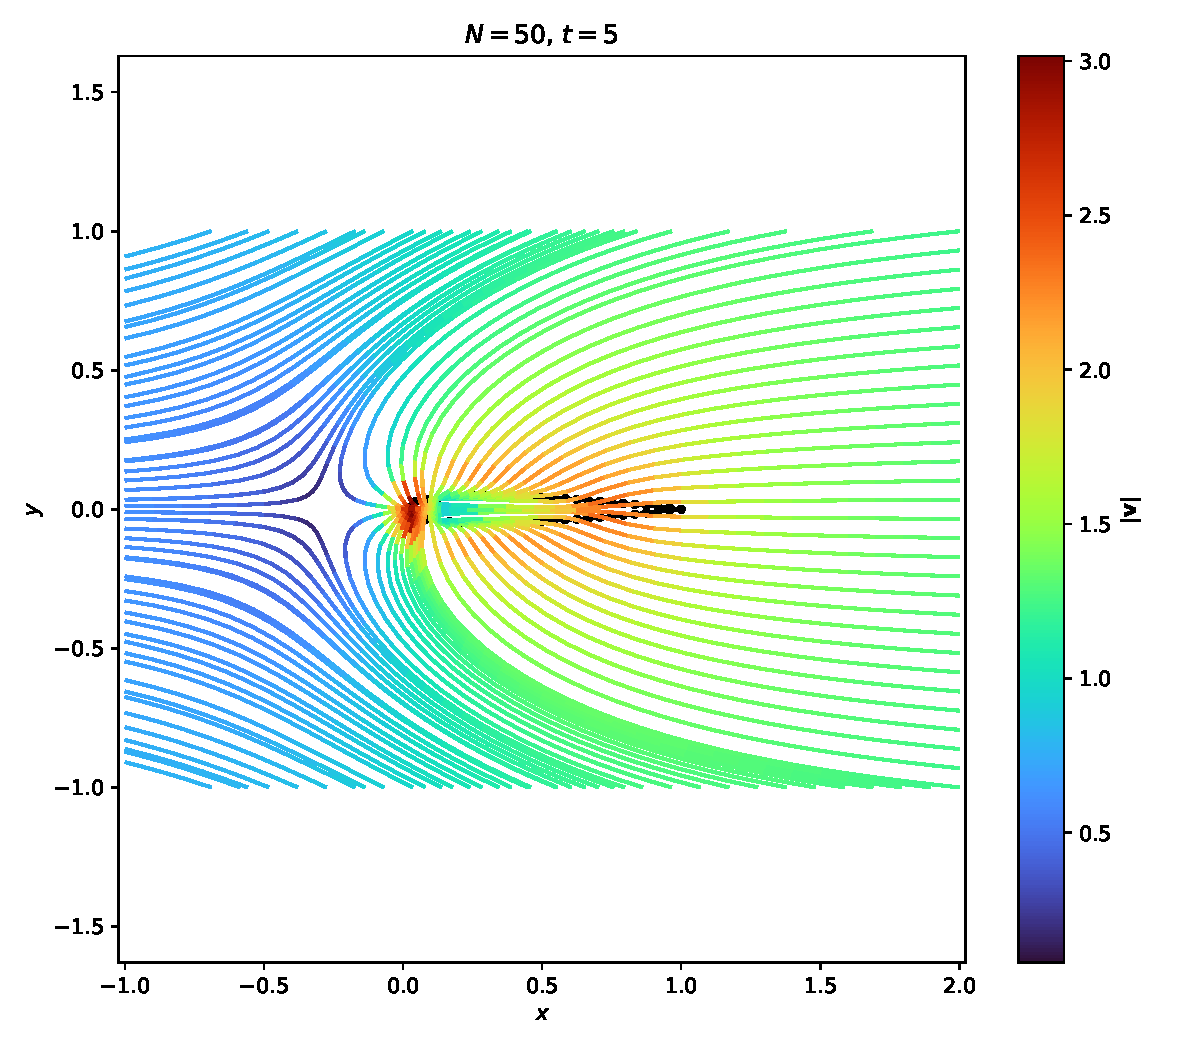
\includegraphics[width=\linewidth]{9.nal_slike/hidro/aeroprofil/NACA_t5_N50_alpha0.pdf}
        \caption{NACA-005}
    \end{subfigure}
    \begin{subfigure}{0.49\textwidth}
        \centering
        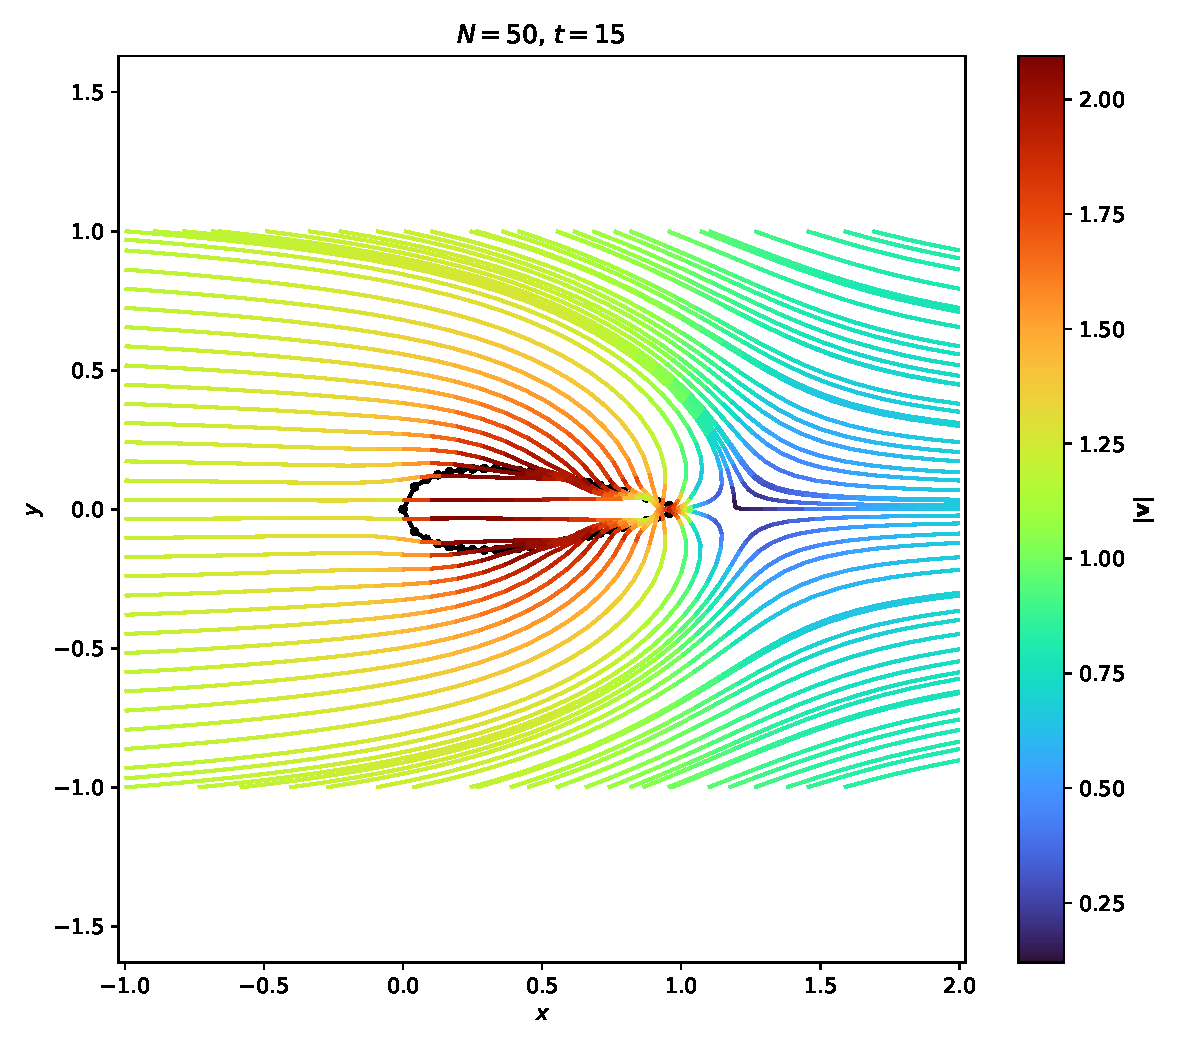
\includegraphics[width=\linewidth]{9.nal_slike/hidro/aeroprofil/NACA_t15_N50_alpha0.pdf}
        \caption{NACA-0015}
    \end{subfigure}
    \caption{NACA aeroprofili v vodoravnem toku -- vpadni kot 0$^\circ$}
\end{figure}

\begin{figure}[H]
    \centering
    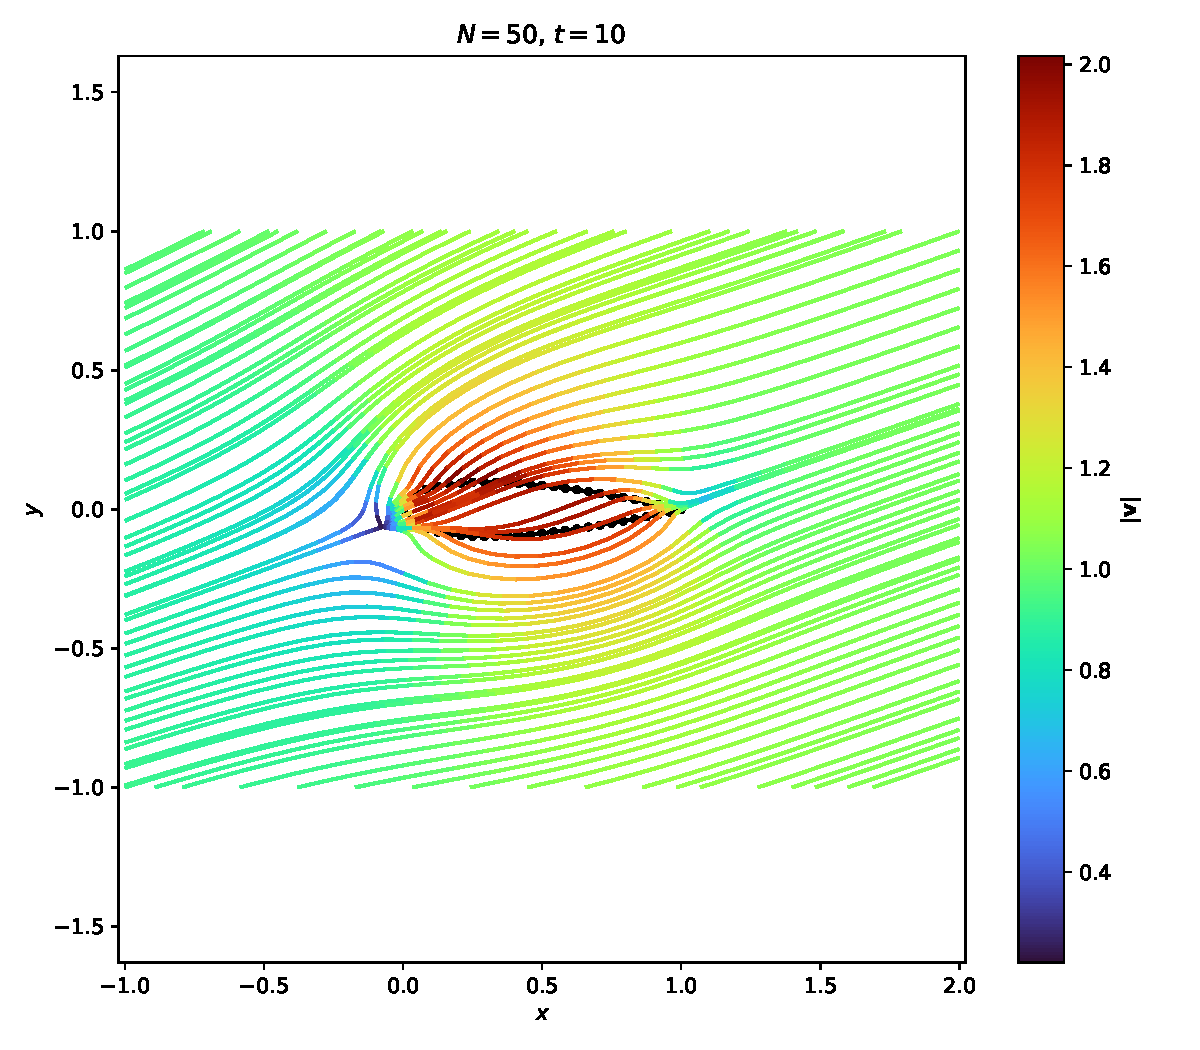
\includegraphics[width=0.45\linewidth]{9.nal_slike/hidro/aeroprofil/NACA_t10_N50_alpha20.pdf}
    \caption{NACA-0010, vpadni kot 20$^\circ$}
\end{figure}

Ker iz mehanike tekočin vem, da obstaja analitična rešitev za tok okoli kroga, katerega je mogoče s kompleksno transformacijo Žukovskega preslikati na različne oblike aeroprofilov
\begin{equation}
    z(\eta) = \frac{1}{2}\,(\eta+\frac{1}{\eta}),\quad \eta(A,B)=A+B\,i+R\,e^{i\,\varphi},
\end{equation}
kjer sta $A$ in $B$ premika na kompleksni ravnini in opisujeta šiljenje repa in krivljenje aeroprofila. Parameter $R$ izračunam na tak način, da se krog na kompleksni ravnin vedno nahaja v točki na realni osi, ki je za 1 iddaljena od izhodišča $R=\sqrt{(1-A)^2+(A^2+B^2)}$. Na tak način dobimo za $-1<A<0$ in $0<B<1$ različne transformacije, ki imajo smiselne oblike aeropfrofilov, in lahko popišemo tudi nesimetrične profile, katere v seriji aeroprofilo NACA sicer popisujeta prvi dve številki.

Kot prvo sem izvedel izračun brez kompleksnih premikov, na elipsi, ki jo dobimo pri transformaciji z $R=1/2$, kjer so rezulatai podobni kot prej. Vendar tudi v tem primeru pri preostalih oblikah prihaja do podobnih degeneracij kot prej.

\begin{figure}[ht]
    \centering
    \begin{subfigure}{0.49\textwidth}
        \centering
        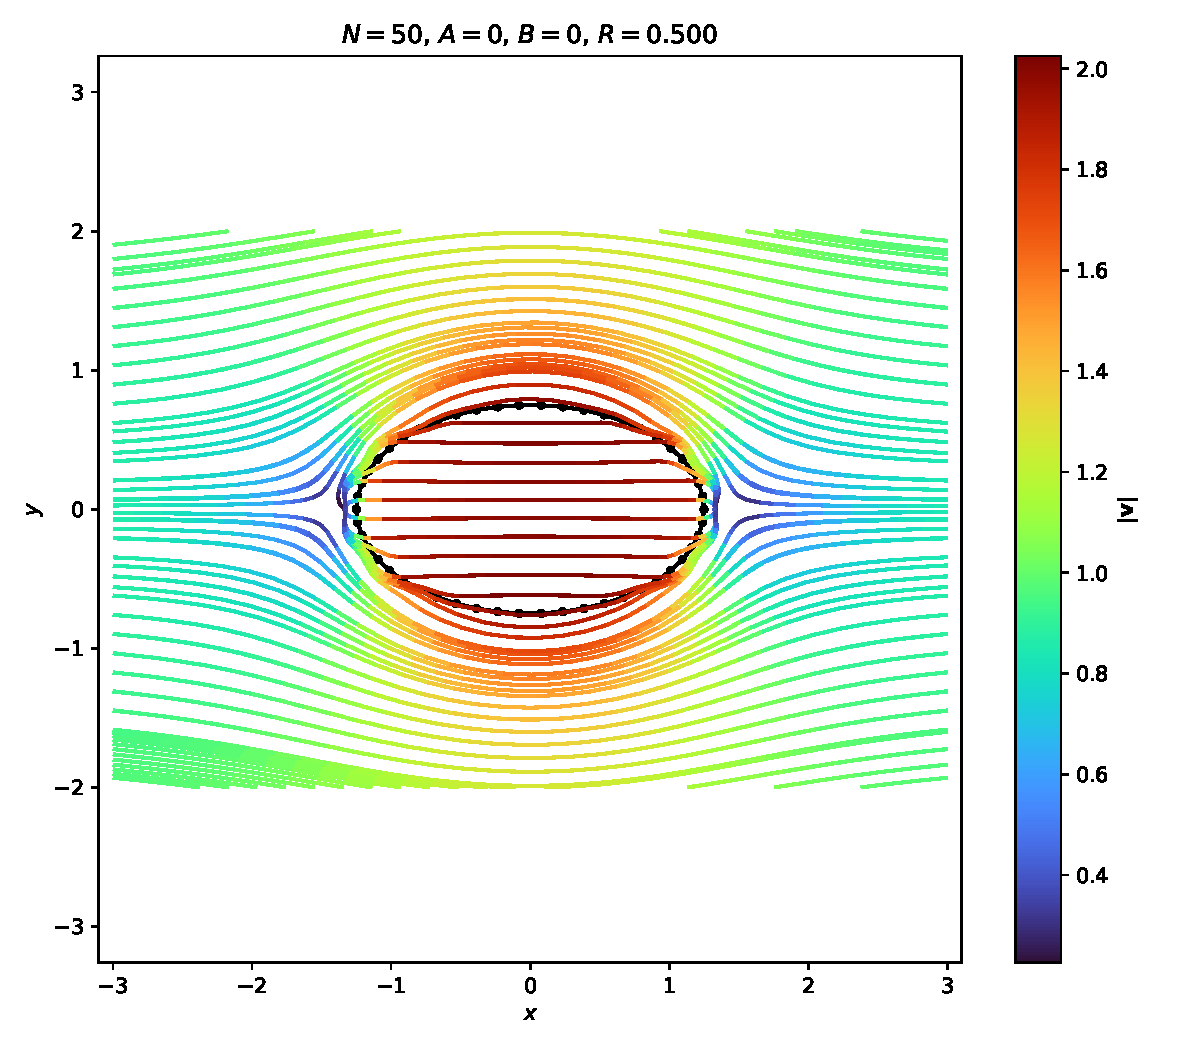
\includegraphics[width=\linewidth]{9.nal_slike/hidro/aeroprofil/zukovski_A0_B0_R0.500_N50_alpha0.pdf}
        \caption{elipsa -- brez premikov v kompleksni ravnini}
    \end{subfigure}
    \begin{subfigure}{0.49\textwidth}
        \centering
        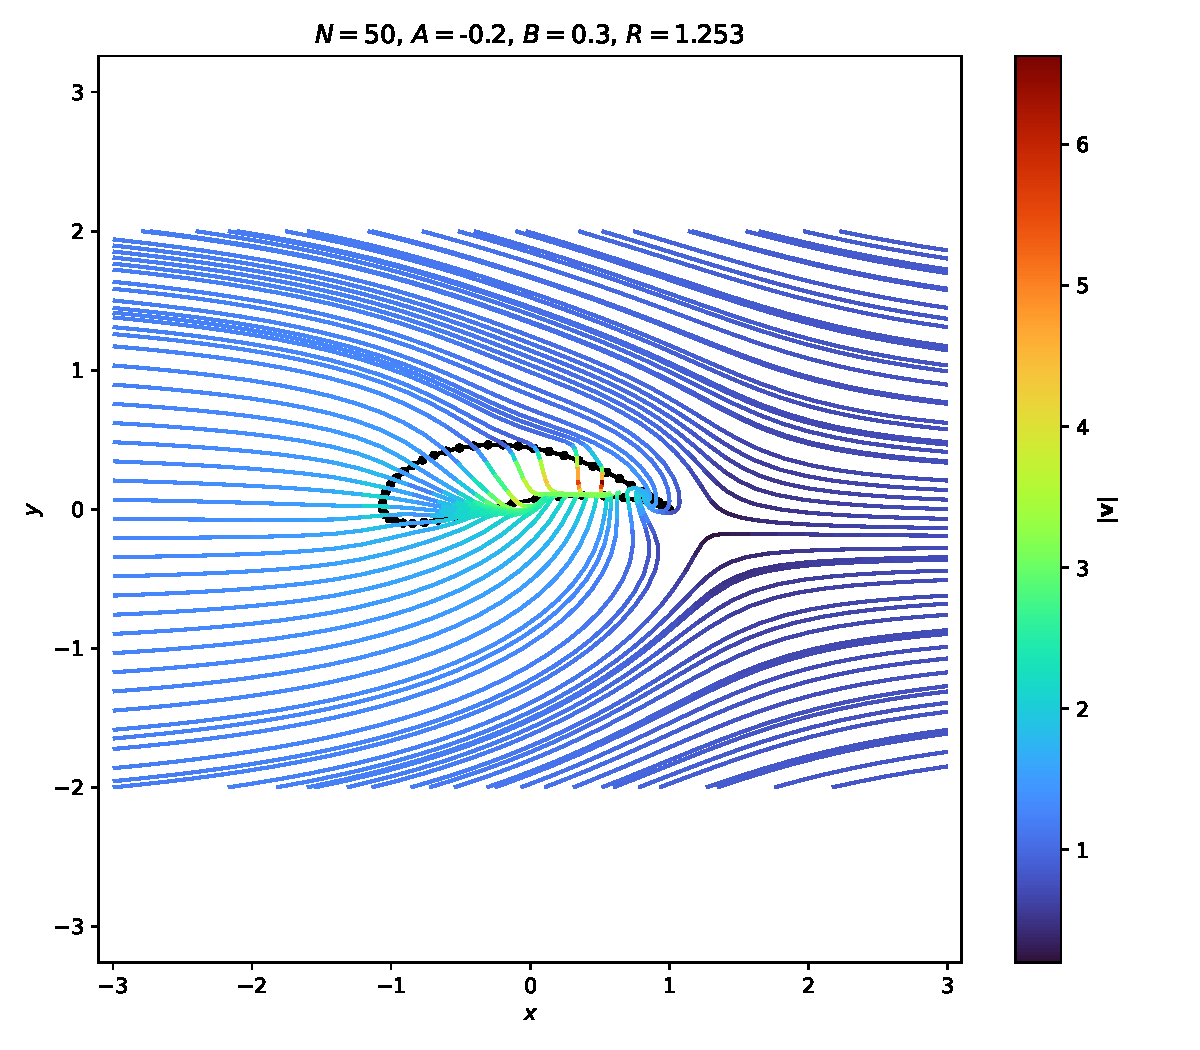
\includegraphics[width=\linewidth]{9.nal_slike/hidro/aeroprofil/zukovski_A-0.2_B0.3_R1.253_N50_alpha0.pdf}
        \caption{kompleksni premik $A=-0.2$, $B=0.3$}
    \end{subfigure}
    \caption{Tok okoli aeroprofilov Žukovskega}
\end{figure}

Še boljši popis transformacije Žukovskega nam nudi polarni zapis kompleksnega števila
\begin{equation}
    z(\eta) = \frac{1}{2}\,(\eta+\frac{1}{\eta}),\quad \eta(r,\phi)=m\,e^{i\,\phi}+R\,e^{i\,\varphi},
\end{equation}
kjer ponovno določimo R tako kot poprej; z vsiljevanjem prečkanja točke (1,0) na kompleksni ravnini tako ustvarjamo oster prehod aeroprofila pri $z=2$, paramter $m$ opisuje odebelitev aeroprofila, $\phi$ pa zakrivljenost.

S pomočjo Mathematice, transformacije Žukovskega in kode, najdene na  \href{https://demonstrations.wolfram.com/JoukowskiAirfoilFlowField/}{internetu}, sem preslikal analitično rešitev za tok okoli kroga na tok okoli aeroprofila Žukovskega na spodnji sliki, kjer rdeča barva predstavlja povečan tlak, modra pa pomanjšan. Sedaj vidim, kakšno napako sem storil, ko sem to računal po MRE!

\begin{figure}[H]
    \centering
    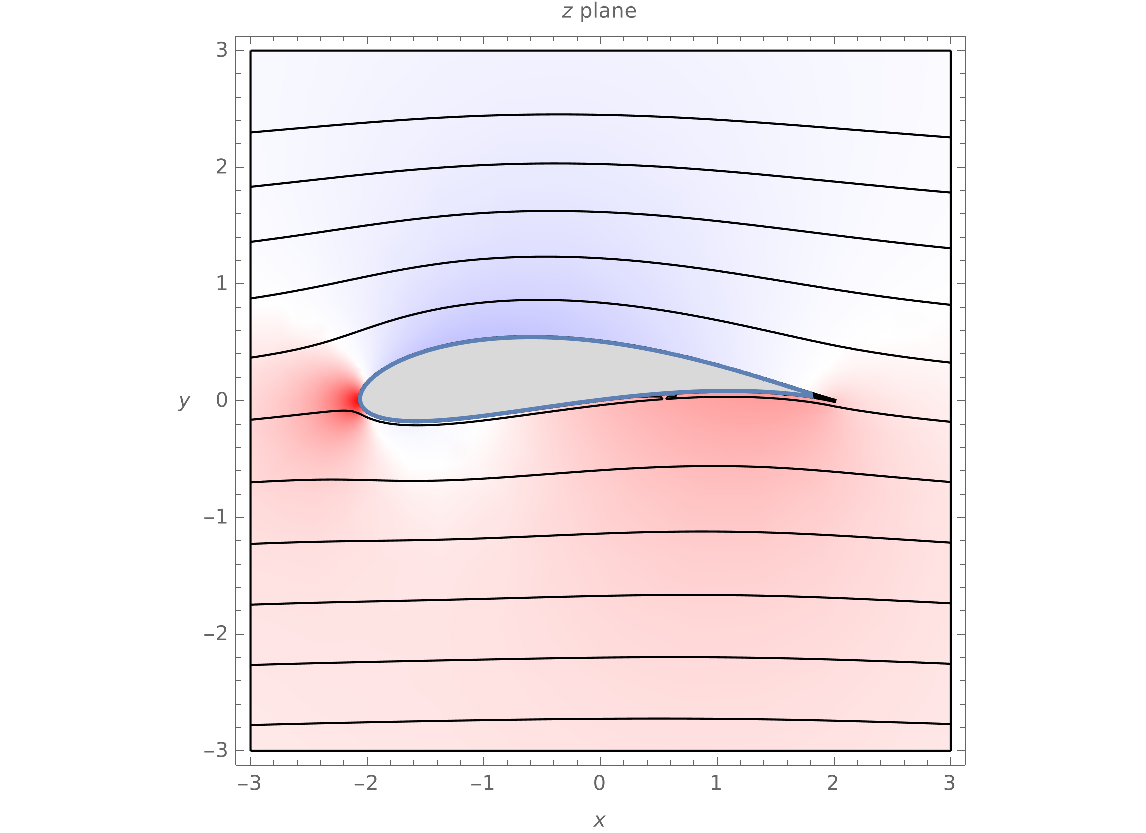
\includegraphics[width=0.65\linewidth]{9.nal_slike/hidro/aeroprofil/zukovski_pressure.pdf}
    \caption{Tlačno polje in tokovnice za aeroprofil Žukovskega pri $m=0.2$ in $\phi=\frac{3\pi}{4}$}
\end{figure}

Preveril sem, če metoda deluje tudi na preostalih aeroprofilih. Star, vendar med modelarji močno priljubljen je še vedno Clark-Y, zz  \href{http://airfoiltools.com/airfoil/details?airfoil=clarky-il}{interneta} sem pridobil podatke zanj, vendar ponovno metoda ne verne zadovoljivih rezulatov, čeprav sem podatke preuredil do te mere, da je profil sklenjen in normale kažejo navzven.

\begin{figure}[ht]
    \centering
    \begin{subfigure}{0.49\textwidth}
        \centering
        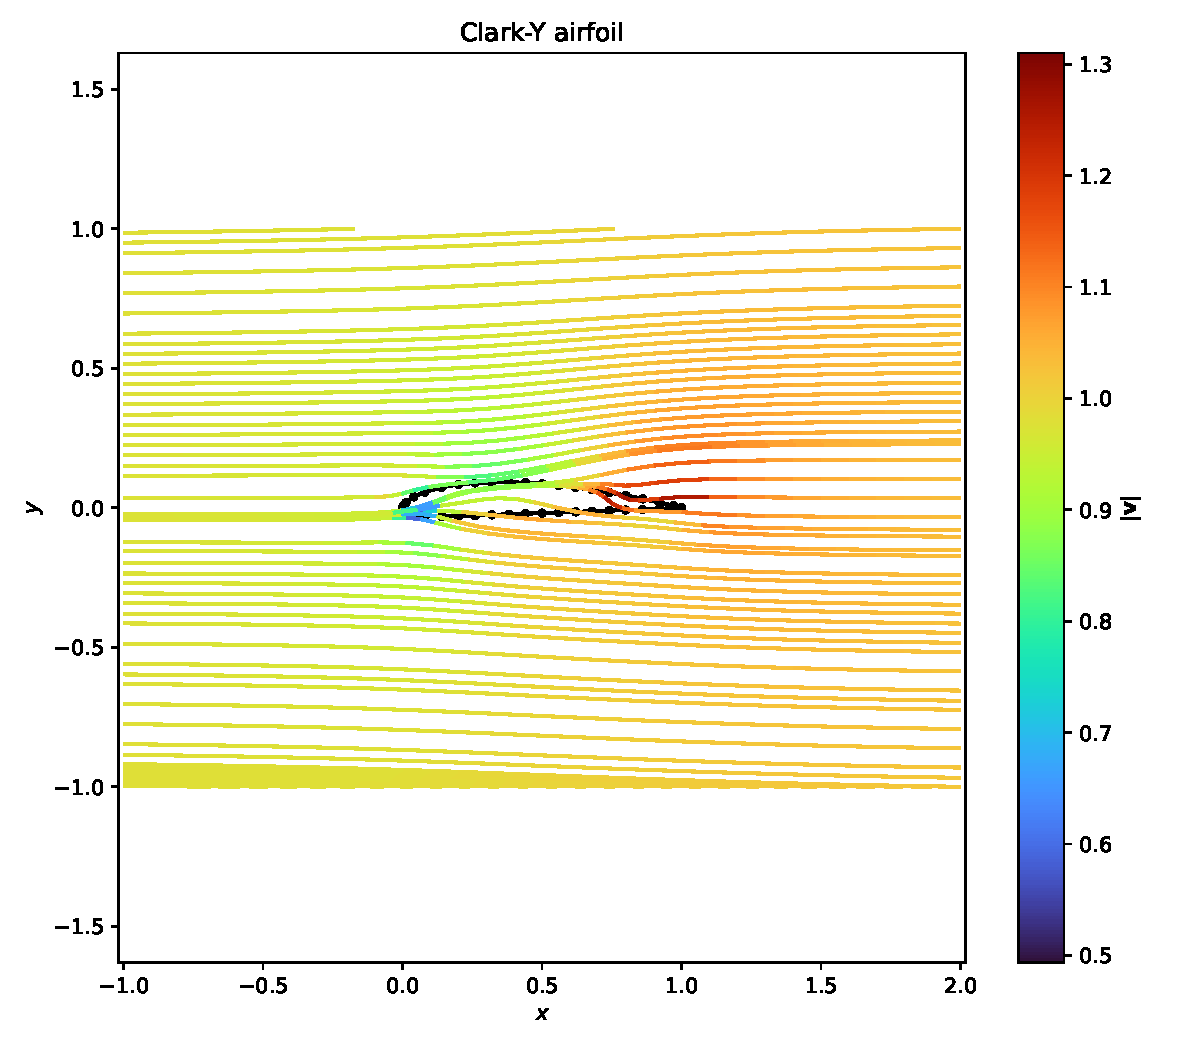
\includegraphics[width=\linewidth]{9.nal_slike/hidro/aeroprofil/clarkY_alpha0.0.pdf}
        \caption{vodoraven tok -- vapdni kot 0$^\circ$}
    \end{subfigure}
    \begin{subfigure}{0.49\textwidth}
        \centering
        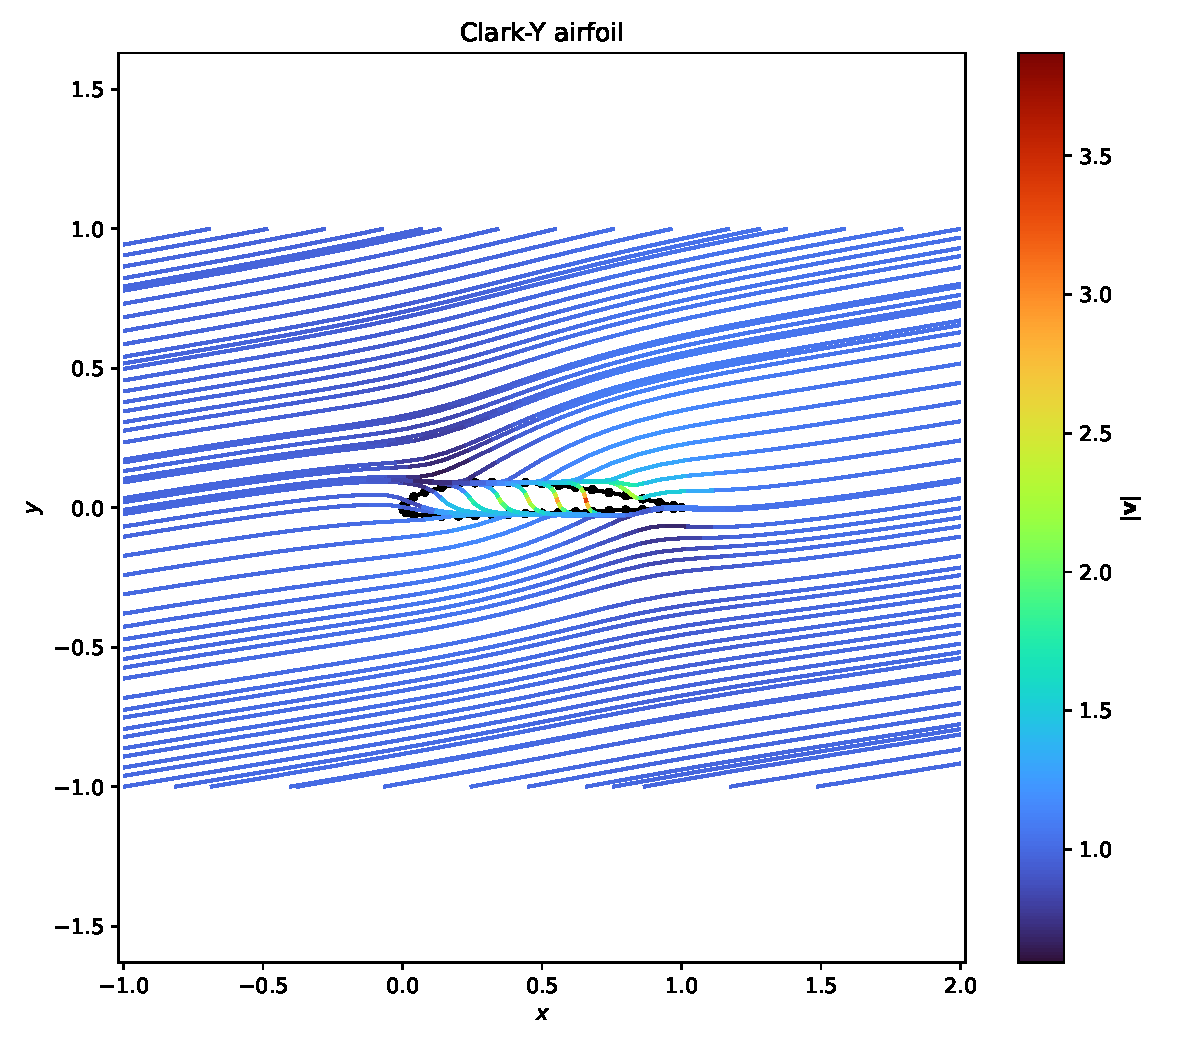
\includegraphics[width=\linewidth]{9.nal_slike/hidro/aeroprofil/clarkY_alpha10.pdf}
        \caption{vpadni kot 10$^\circ$}
    \end{subfigure}
    \caption{Tok okoli aeroprofila Clark Y}
\end{figure}

Z malo iskanja po internetu sem na portalu Wolfram Demostrations Project našel pogram, ki po isti metodi za aeroprofile v bazi podatkov izračuna potencialni tok. Za Clark-Y je rezultat prikazan na spodnji sliki, prav tako pa je mogoče s tem precej dobro izračunati tok okoli NACA aeroprofilov. Očitno je nekaj narobe v moji kodi, vendar za eliptične oblike pa je delovala zadovoljivo, zato se nisem lotil iskanja vzroka!

\begin{figure}[H]
    \centering
    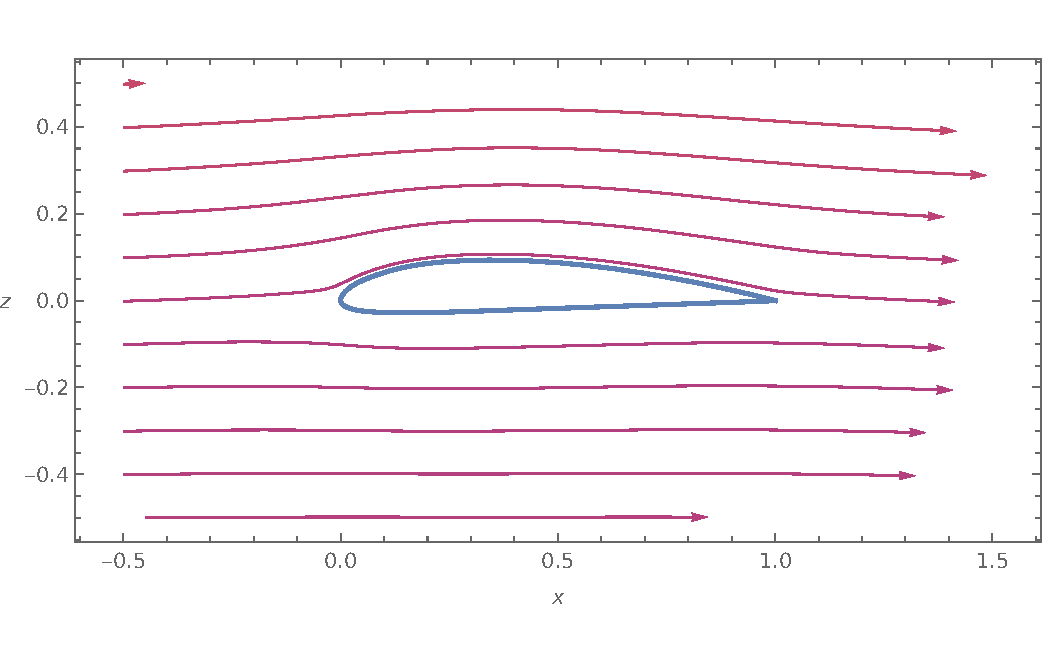
\includegraphics[width=0.65\linewidth]{9.nal_slike/hidro/aeroprofil/clarkY-mathematica.pdf}
    \caption{Tokovnice okoli Clark-Y aeroprofila, izračunano z \href{https://demonstrations.wolfram.com/PotentialFlowOverAnAirfoilSpecifiedByNumericalDataFile/}{Demonstracijsko kodo}}
\end{figure}

V dinamiki tekočin se sicer uporabljajo metode, ki temeljijo na reševanji Navier-Stokesovih enačb. Pri predmetu Računalniška dinamika tekočin smo se naučili izdelati C-blok stukturirano mrežo za turbulenten tok, zato je na spodnji sliki prikazan izračun za NACA-23018 aeroprofil, kjer so enačbe rešene po metodi končnih volumnov in sklopljene s PISO rešitvenim postopkom. Za diskretizacijo je uporabljena privetrnea shema 2.reda, turbulenten režim pa je popisan z k-$\varepsilon$ modelom in y$^+$ stensko funkcijo ob aeroprofilu.

\begin{figure}[H]
    \centering
    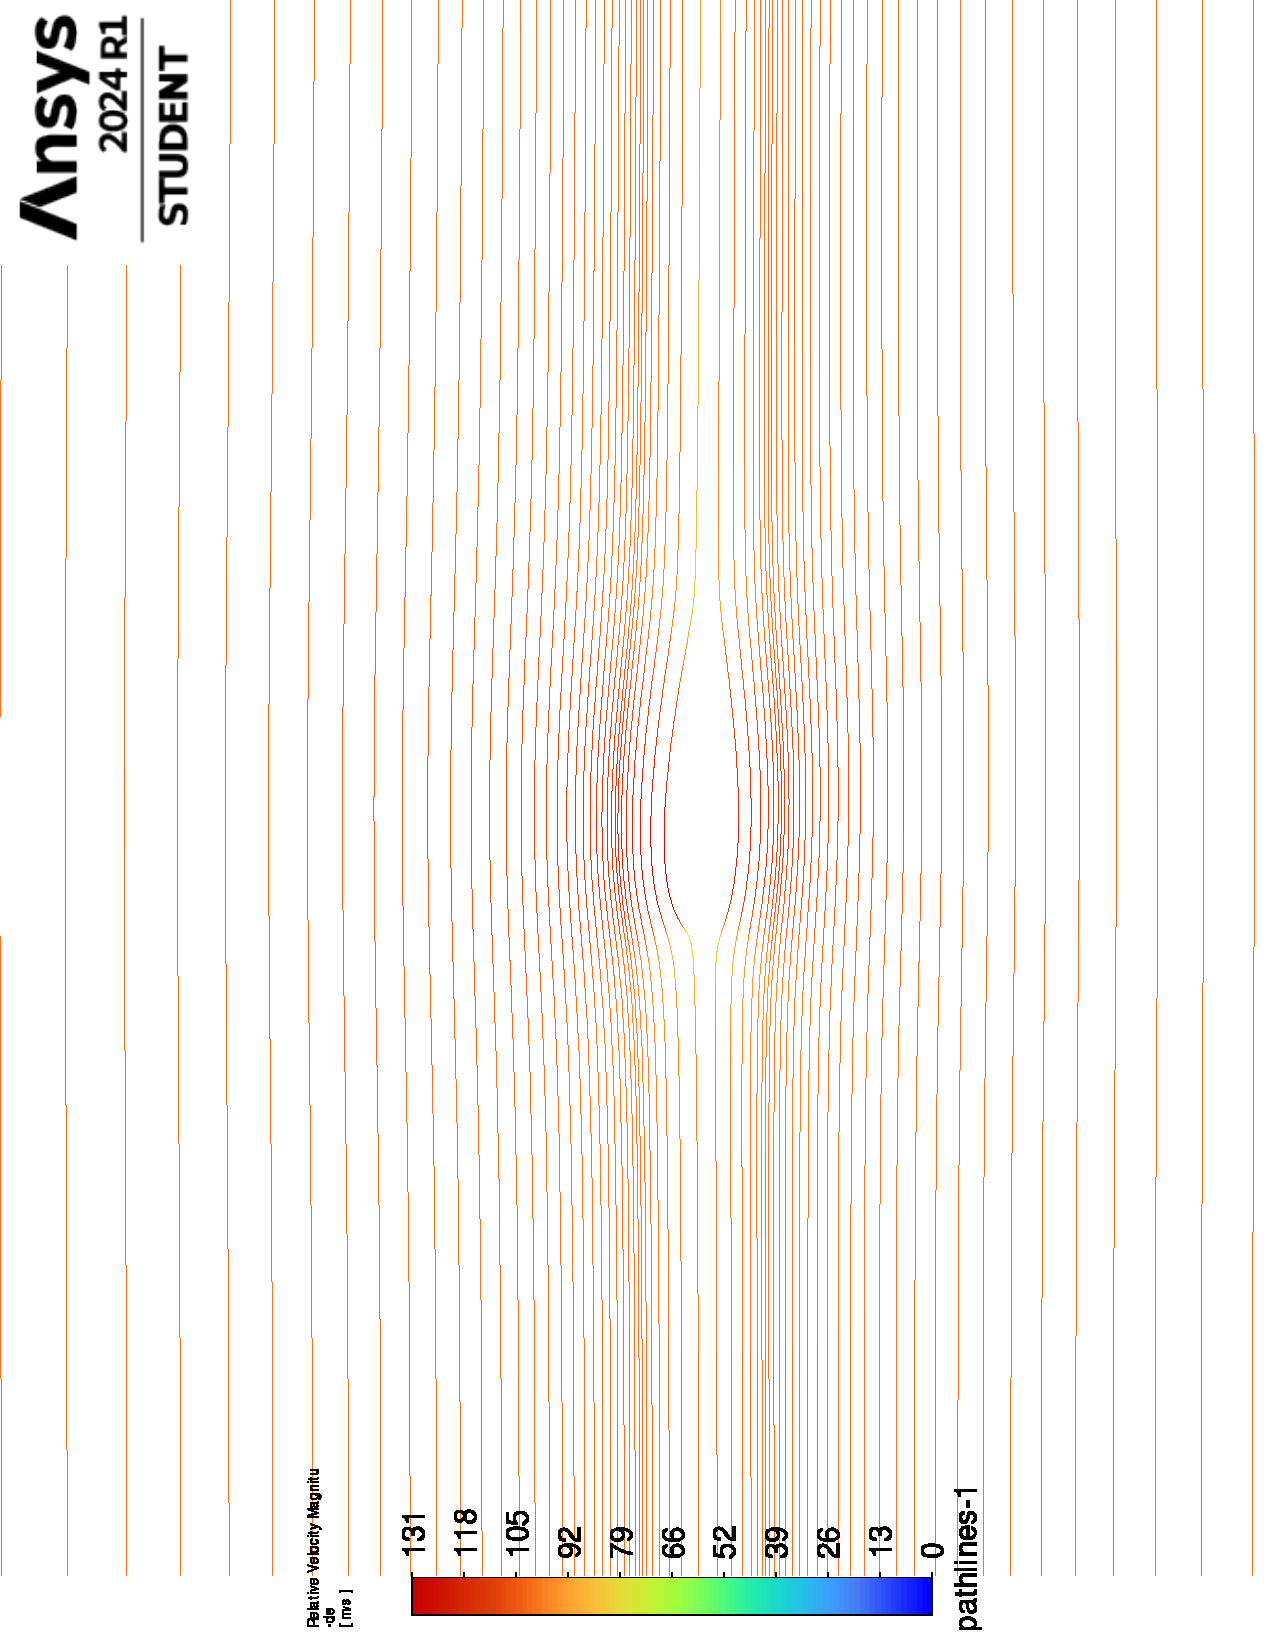
\includegraphics[angle=-90,origin=c,width=\linewidth]{9.nal_slike/hidro/aeroprofil/naca23018_rdt.pdf}
    \caption{Tok okoli NACA23018 aeroprofila, izračunano v Ansys Fluent}
\end{figure}